\documentclass[german]{spicker}

\addbibresource{ds.bib}

\title{Einführung in Data Science}
\author{Patrick Gustav Blaneck}
\makeindex[intoc]
\makeindex[intoc, name=Beispiele,title=Beispiele]

\begin{document}
\maketitle
\tableofcontents
\newpage

\section{Explorative Datenanalyse}

\begin{defi}{Explorative Datenanalyse}
    Die \emph{explorative Datenanalyse (EDA)}, eine Weiterentwicklung der deskriptiven Statistik zur Analyse von Daten, arbeitet mehr induktiv: Mit ihren Methoden soll Neues entdeckt, sollen Vermutungen generiert, Besonderheiten erkannt und Sachverhalte dargestellt werden.

    Sie untersucht und begutachtet Daten, von denen nur ein geringes Wissen über deren Zusammenhänge vorliegt. Viele EDA-Techniken werden im Data-Mining eingesetzt.

    Ziele der explorativen Datenanalyse sind:
    \begin{itemize}
        \item Annahmen (\emph{Hypothesen}) über die Ursache und den Grund der beobachteten Daten zu bilden
        \item Annahmen \emph{einzuschätzen}, worauf statistische Inferenz basieren kann
        \item Die Auswahl von passenden statistischen \emph[Werkzeugen und Techniken] zu unterstützen
    \end{itemize}

    \centering
    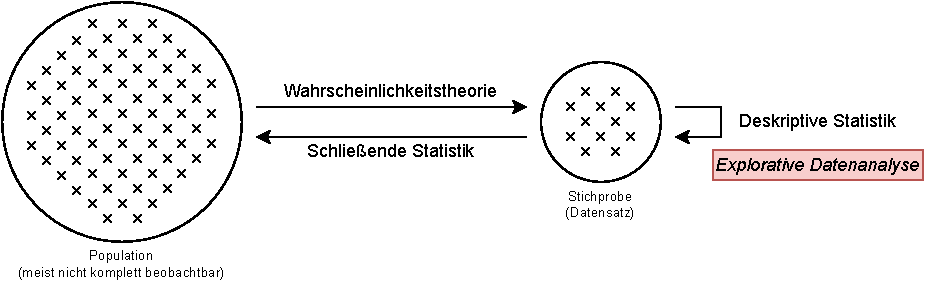
\includegraphics[width=.9\textwidth]{includes/figures/defi_explorative_datenanalyse.pdf}
\end{defi}

\subsection{Lageparameter}

\begin{defi}{Arithmetisches Mittel}
    Das \emph{arithmetische Mittel} berechnet man, indem man die Summe der betrachteten Zahlen durch ihre Anzahl teilt und beschreibt damit das Zentrum einer Verteilung durch einen numerischen Wert und stellt einen Lageparameter dar.

    Es gilt:
    \begin{itemize}
        \item Für Stichproben in einer Urliste, wobei $x_i$ die Ausprägung des $i$-ten Elements darstellt:
              \[
                  \conj{x} = \frac{1}{n} \sum_{i=1}^n x_i
              \]
        \item Für eine unklassierte Häufigkeitstabelle, wobei $h_i$ die relative Häufigkeit des $i$-ten Elements $a_i$ darstellt:
              \[
                  \conj{x} = \sum_{i=1}^n h_i \cdot a_i
              \]
        \item Für eine klassierte Häufigkeitstabelle, wobei $h_i$ die relative Häufigkeit der $i$-ten Klasse $A_i$, und $\alpha_i$ die Klassenmitte darstellt:
              \[
                  \conj{x} \approx \sum_{i=1}^n h_i \cdot \alpha_i
              \]
    \end{itemize}
\end{defi}

\begin{bonus}{Median}
    Der \emph{Median} der Messwerte einer Urliste ist derjenige Messwert, der genau \enquote{in der Mitte} steht, wenn man die Messwerte der Größe nach sortiert.

    Im Allgemeinen teilt ein Median einen Datensatz, eine Stichprobe oder eine Verteilung so in zwei gleich große Teile, dass die Werte in der einen Hälfte nicht größer als der Medianwert sind und in der anderen nicht kleiner.

    Es gilt:
    \begin{itemize}
        \item Für Stichproben in einer \emph{sortierten} Urliste, wobei $x_i$ die Ausprägung des $i$-ten Elements darstellt:
              \[
                  \tilde{x} =
                  \begin{cases}
                      x_{\nicefrac{(n+1)}{2}}                                                  & \text{falls $n$ ungerade} \\
                      \frac{1}{2} \left( x_{\nicefrac{n}{2}} + x_{\nicefrac{(n+1)}{2}} \right) & \text{falls $n$ gerade}
                  \end{cases}
              \]
        \item Für eine unklassierte Häufigkeitstabelle, wobei $H_i$ die kumulierte relative Häufigkeit bis zum $i$-ten Element $a_i$ darstellt:
              \begin{itemize}
                  \item $\tilde{x}$ ist das Merkmal $a_i$, bei dem $H_i = 0.5$ zum ersten Mal überschritten wird.
              \end{itemize}
        \item Für eine klassierte Häufigkeitstabelle, wobei $H_i$ die kumulierte relative Häufigkeit bis zur $i$-ten Klasse $A_i$ darstellt:
              \begin{itemize}
                  \item $\tilde{x}$ befindet sich in der \emph{Einfallsklasse}, die zum ersten Mal $H_i = 0.5$ erreicht.
                  \item Sei $A_j = \left( a_j, b_j \right]$ die Einfallsklasse.
                        Dann gilt:\footnote{Siehe \emph{Quantil (empirisch)} für mehr Informationen.}
                        \[
                            \tilde{x} = x_{0.5} = a_j + \frac{0.5 - H_{j-1}}{H_{j} - H_{j-1}} \cdot (b_j - a_j)
                        \]
              \end{itemize}
    \end{itemize}
\end{bonus}

\begin{defi}{Quantil (empirisch)}
    Für jede Zahl $p$ zwischen 0 und 1 teilt ein \emph{empirisches p-Quantil} die Stichprobe so, dass ein Anteil der Stichprobe von $p$ kleiner als das empirische $p$-Quantil ist und ein Anteil von $1-p$ der Stichprobe größer als das empirische $p$-Quantil ist.

    Es gilt:
    \begin{itemize}
        \item Für Stichproben in einer \emph{sortierten} Urliste, wobei $x_i$ die Ausprägung des $i$-ten Elements darstellt:
              \[
                  x_p =
                  \begin{cases}
                      \frac{1}{2} \left( x_{n \cdot p} + x_{n \cdot p + 1} \right) & \text{falls $n \cdot p$ ganzzahlig}       \\
                      x_{\floor{n \cdot p + 1}}                                    & \text{falls $n \cdot p$ nicht ganzzahlig} \\
                  \end{cases}
              \]
        \item Für eine unklassierte Häufigkeitstabelle, wobei $h_i$ die relative Häufigkeit des $i$-ten Elements $a_i$ darstellt:
              \begin{itemize}
                  \item $x_p$ ist das Merkmal $a_i$, bei dem $H_i = p$ zum ersten Mal überschritten wird.
              \end{itemize}
        \item Für eine klassierte Häufigkeitstabelle, wobei $H_i$ die kumulierte relative Häufigkeit bis zur $i$-ten Klasse $A_i$ darstellt:
              \begin{itemize}
                  \item $x_p$ befindet sich in der \emph{Einfallsklasse}, die zum ersten Mal $H_i = p$ erreicht.
                  \item Sei $A_j = \left( a_j, b_j \right]$ die Einfallsklasse.
                        Dann gilt:
                        \[
                            x_p = a_j + \frac{p - H_{j-1}}{H_{j} - H_{j-1}} \cdot (b_j - a_j)
                        \]
              \end{itemize}
    \end{itemize}
\end{defi}

\subsection{Streuungsparameter}

\begin{defi}{Empirische Varianz}
    Die \emph{empirische Varianz} bzw. \emph{Stichprobenvarianz}  ist eine statistische Angabe für die Streubreite von Werten einer Stichprobe.

    Sie gehört zu den Streuungsmaßen und beschreibt die mittlere quadratische Abweichung der einzelnen Messwerte vom empirischen Mittelwert.

    Sie stellt damit eine Art durchschnittliches Abweichungsquadrat dar.

    Die positive Wurzel der empirischen Varianz ist die \emph{empirische Standardabweichung}.
    Die empirische Standardabweichung stellt das gebräuchlichste Streuungsmaß dar.

    Es gilt:
    \begin{itemize}
        \item Für Stichproben in einer Urliste, wobei $x_i$ die Ausprägung des $i$-ten Elements darstellt:
              \[
                  s^2 = \frac{1}{n-1} \sum_{i=1}^{n} (x_i - \conj{x})^2 = \frac{1}{n-1} \left( \sum_{i=1}^{n} x_i^2 - n\cdot \conj{x}^2 \right)
              \]
        \item Für eine unklassierte Häufigkeitstabelle, wobei $n_j$ die absolute Häufigkeit des $j$-ten Elements $a_j$ darstellt:
              \[
                  s^2 = \frac{1}{n-1} \sum_{j=1}^{m} (a_j - \conj{x})^2 \cdot n_j = \frac{1}{n-1} \left( \sum_{j=1}^{m} a_j^2 \cdot n_j - \conj{x}^2 \right)
              \]
        \item Für eine klassierte Häufigkeitstabelle, wobei $n_j$ die absolute Häufigkeit der $j$-ten Klasse $A_j$, und $\alpha_j$ die Klassenmitte darstellt:
              \[
                  s^2 \approx \frac{1}{n-1} \sum_{j=1}^{m} \alpha_j^2 \cdot n_j - \frac{1}{n(n-1)} \left( \sum_{j=1}^{m} \alpha_j \cdot n_j \right)^2
              \]
    \end{itemize}

    Insgesamt gilt natürlich jeweils für die empirische Standardabweichung:
    \[
        s = \sqrt{s^2}
    \]
\end{defi}

\begin{defi}{Quartilsabstand}
    Der \emph{Quartilsabstand} bzw. \emph{Interquartilsabstand} $Q$ gibt für eine sortierte Stichprobe an, wie breit das Intervall ist, in dem die mittleren 50\% der Stichprobeelemente liegen.

    Es gilt:
    \[
        Q = x_{0.75} - x_{0.25}
    \]
\end{defi}

\subsection{Deskriptive Statistik}

\begin{defi}{Box-Plot}
    \begin{wrapfigure}{r}{0.5\textwidth}
        \centering
        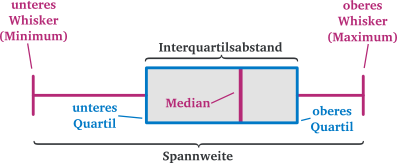
\includegraphics[width=0.45\textwidth]{includes/figures/definition_boxplot.png}
    \end{wrapfigure}%
    %
    Der \emph{Box-Plot} ist ein Diagramm, das zur grafischen Darstellung der Verteilung eines mindestens ordinalskalierten Merkmals verwendet wird.

    Es fasst dabei verschiedene robuste Streuungs- und Lagemaße in einer Darstellung zusammen.

    Ein Box-Plot soll schnell einen Eindruck darüber vermitteln, in welchem Bereich die Daten liegen und wie sie sich über diesen Bereich verteilen. Deshalb werden alle Werte der sogenannten Fünf-Punkte-Zusammenfassung, also der Median, die zwei Quartile und die beiden Extremwerte, dargestellt.

    Zusammengefasst lassen sich folgende Kennwerte ablesen:

    \begin{center}
        \begin{tabular}{|l|p{0.4\linewidth}|p{0.3\linewidth}|}
            \hline
            Kennwert        & Beschreibung                                                                          & Lage im Box-Plot                                   \\
            \hline
            \hline
            Minimum         & Kleinster Datenwert des Datensatzes                                                   & Ende eines Whiskers oder entferntester Ausreißer   \\
            \hline
            Unteres Quartil & Die kleinsten 25\% der Datenwerte sind kleiner als dieser oder gleich diesem Kennwert & Beginn der Box                                     \\
            \hline
            Oberes Quartil  & Die kleinsten 75\% der Datenwerte sind kleiner als dieser oder gleich diesem Kennwert & Ende der Box                                       \\
            \hline
            Maximum         & Größter Datenwert des Datensatzes                                                     & Ende eines Whiskers oder entferntester Ausreißer   \\
            \hline
            Spannweite      & Gesamter Wertebereich des Datensatzes                                                 & Länge des gesamten Box-Plots (inklusive Ausreißer) \\
            \hline
            Quartilsabstand & Wertebereich, in dem sich die mittleren 50\% der Daten befinden                       & Ausdehnung der Box                                 \\
            \hline
        \end{tabular}
    \end{center}
\end{defi}

\begin{bonus}{5 Number Summary}
    TODO
\end{bonus}

\begin{defi}{Histogramm}
    TODO
\end{defi}

\subsection{Visualisierung}

\begin{defi}{Regeln für Visualisierungen}
    Regeln nach Edward Tufte:
    \begin{itemize}
        \item Maximieren des Daten-Druckerschwärze-Verhältnis (so wenig Druckerschwärze für soviele Daten wie möglich)
        \item Minimieren des Lügenfaktors
        \item Minimieren des \enquote{Chartjunks} (keine visuellen Spielereien)
        \item Nutzen von angemessenen Skalen, Achsenbeschriftungen
        \item Farbe zum Darstellen von Eigenschaften der Daten, nicht für Ästhetik oder Kommunikation
    \end{itemize}
\end{defi}

\begin{bonus}{Notwendigkeit von Visualisierungen}
    Für unterschiedliche Datensätze können ähnliche Kennzahlen entstehen.

    Aus diesem Grund werden Visualisierungen für die Erkundung von Daten benötigt.
\end{bonus}

\begin{bonus}{Auswahl einer Diagrammart}
    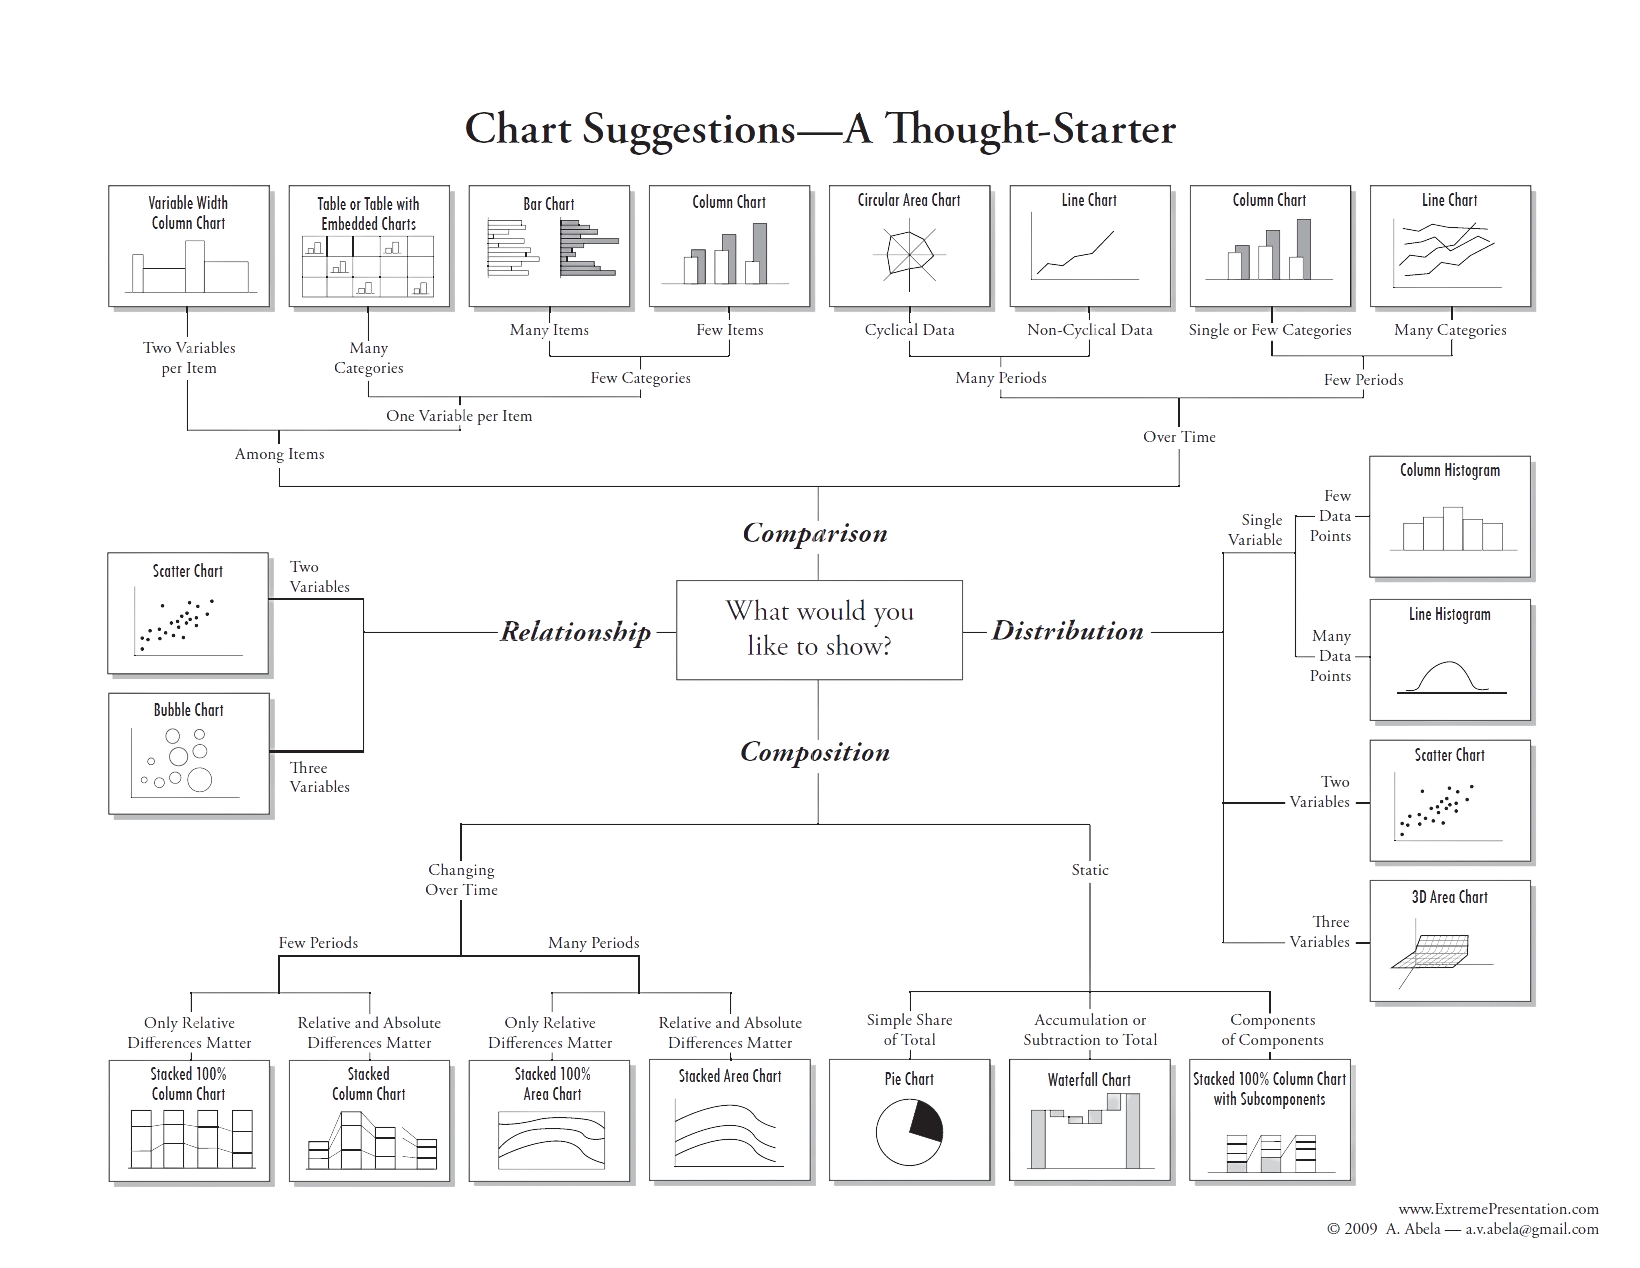
\includegraphics[width=\textwidth]{includes/figures/bonus_chart_suggestion.png}
\end{bonus}

\begin{example}{Anscombe-Quartett}
    Das \emph{Anscombe-Quartett} besteht aus vier Mengen von Datenpunkten, die nahezu identische einfache statistische Eigenschaften haben, aber aufgetragen sehr verschieden aussehen.

    Für die vier Punktmengen gilt:
    \begin{itemize}
        \item Mittelwert von $x$ in jedem Fall: 9 (exakt)
        \item Varianz von $x$ in jedem Fall: 11 (exakt)
        \item Mittelwert von $y$ in jedem Fall: 7.50 (auf 2 Stellen)
        \item Varianz von $y$ in jedem Fall: 4.122 oder 4.127 (auf 3 Stellen)
        \item Korrelation zwischen $x$ und $y$ in jedem Fall: 0.816 (auf 3 Stellen)
        \item Lineare Regression in jedem Fall: $y = 3.00 + 0.500x$ (auf 2 bzw. 3 Stellen)
    \end{itemize}

    Die Datenpunkte sind gegeben wie folgt:

    \begin{center}
        \begin{tabular}{|l|l||l|l||l|l||l|l|}
            \hline
            \multicolumn{2}{|l||}{Reihe 1} & \multicolumn{2}{l||}{Reihe 2} & \multicolumn{2}{l||}{Reihe 3} & \multicolumn{2}{l|}{Reihe 4}                               \\ \hline
            x                              & y                             & x                             & y                            & x    & y     & x    & y     \\ \hline\hline
            4.0                            & 4.26                          & 4.0                           & 3.10                         & 4.0  & 5.39  & 8.0  & 5.25  \\ \hline
            5.0                            & 5.68                          & 5.0                           & 4.74                         & 5.0  & 5.73  & 8.0  & 5.56  \\ \hline
            6.0                            & 7.24                          & 6.0                           & 6.13                         & 6.0  & 6.08  & 8.0  & 5.76  \\ \hline
            7.0                            & 4.82                          & 7.0                           & 7.26                         & 7.0  & 6.42  & 8.0  & 6.58  \\ \hline
            8.0                            & 6.95                          & 8.0                           & 8.14                         & 8.0  & 6.77  & 8.0  & 6.89  \\ \hline
            9.0                            & 8.81                          & 9.0                           & 8.77                         & 9.0  & 7.11  & 8.0  & 7.04  \\ \hline
            10.0                           & 8.04                          & 10.0                          & 9.14                         & 10.0 & 7.46  & 8.0  & 7.71  \\ \hline
            11.0                           & 8.33                          & 11.0                          & 9.26                         & 11.0 & 7.81  & 8.0  & 7.91  \\ \hline
            12.0                           & 10.84                         & 12.0                          & 9.13                         & 12.0 & 8.15  & 8.0  & 8.47  \\ \hline
            13.0                           & 7.58                          & 13.0                          & 8.74                         & 13.0 & 12.74 & 8.0  & 8.84  \\ \hline
            14.0                           & 9.96                          & 14.0                          & 8.10                         & 14.0 & 8.84  & 19.0 & 12.50 \\ \hline
        \end{tabular}
    \end{center}

    Die Reihen sind offensichtlich komplett verschieden:

    \centering
    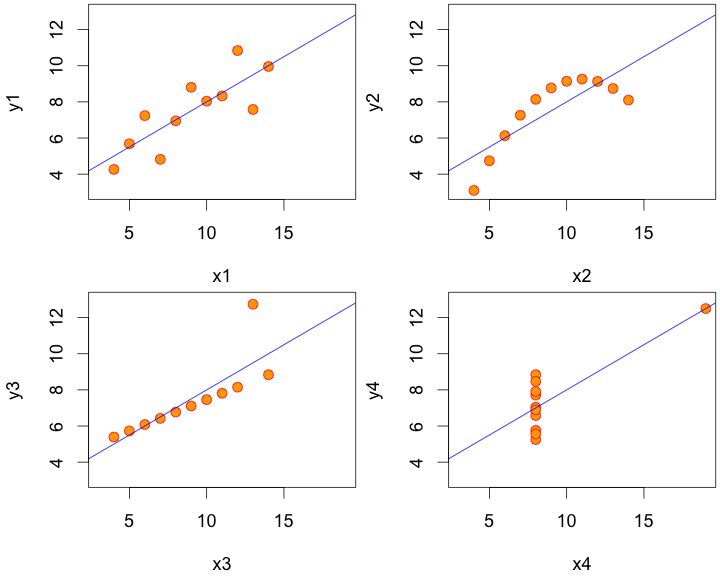
\includegraphics[width=.7\textwidth]{includes/figures/example_anscombe.png}
\end{example}
\section{Multivariate Explorative Analyse}

\begin{defi}{Multivariate Explorative Analyse}
    Mit Hilfe von \emph{multivariaten Verfahren} werden in der multivariaten Statistik mehrere statistische Variablen oder Zufallsvariablen (\emph{Features}) zugleich untersucht.

    In der univariaten Analyse hingegen wird jede Variable einzeln analysiert.
\end{defi}

\begin{defi}{Scatter-Plot}
    TODO
\end{defi}


\begin{defi}{Bubble Chart}
    TODO
\end{defi}

\subsection{Zusammenhangsmaße (Interdependenzmaße)}

\begin{defi}{Pearsons Korrelationskoeffizient}
    Der \emph{Person'sche Korrelationskoeffizient} ist ein Maß für den Grad des linearen Zusammenhangs zwischen zwei Zufallsvariablen.
    Er kann Werte zwischen $-1$ und $+1$ annehmen.

    Bei einem Wert von $+1$ (bzw. $-1$) besteht ein vollständig positiver (bzw. negativer) linearer Zusammenhang zwischen den betrachteten Merkmalen.
    Wenn der Korrelationskoeffizient den Wert $0$ aufweist, hängen die beiden Merkmale überhaupt nicht linear voneinander ab.

    Allerdings können diese ungeachtet dessen in nichtlinearer Weise voneinander abhängen.

    Damit ist der Korrelationskoeffizient kein geeignetes Maß für die (reine) stochastische Abhängigkeit von Merkmalen.

    Der Pearson'sche Korrelationskoeffizient ist definiert durch
    \[
        \rho_{\text{PE}} := \frac{\Cov(X, Y)}{\sigma_X \cdot \sigma_Y} = \frac{\sum_{i=1}^{n}{(x_i - \conj{x})(y_i - \conj{y})}}{\sqrt{\sum_{i=1}^{n}(x_i - \conj{x})^2 \sum_{i=1}^{n}(y_i - \conj{y})^2}}
    \]
\end{defi}

\begin{defi}{Spearmans Korrelationskoeffizient}
    Der \emph{Spearmans'sche Korrelationskoeffizient} entspricht dem Pearson'schen Korrelationskoeffizient, bezieht sich allerdings auf die Ränge der Werte und charakterisiert somit die Stärke des monotonen Zusammenhangs.

    Seien die Werte $x_i$ einer Stichprobe der Größe $n$ des Merkmals $X$ geordnet:
    \[
        x_1 \leq x_2 \leq \ldots \leq x_n
    \]

    Dann ist der Rang eines Wertes definiert als:
    \[
        \rang(x_i) = i
    \]

    Bei identischen Werten ist die Rangvergabe nicht mehr eindeutig und es wird der Durchschnittsrang gebildet.\footnote{D. h.: identischen Werten wird als Rang das arithmetische Mittel der infrage kommenden Ränge zugewiesen.}

    Es gilt also:
    \[
        \rho_{\text{SP}} :=  = \frac{\sum{(\rang(x_i) - \conj{\rang}_X)(\rang(y_i) - \conj{\rang}_Y)}}{\sqrt{\sum(\rang(x_i) - \conj{\rang}_X)^2 \sum(\rang(y_i) - \conj{\rang}_Y)^2}}
    \]

    mit folgenden Mittelwerten der Ränge:
    \[
        \conj{\rang}_X = \frac{1}{n} \sum_{i=1}^{n} \rang(x_i) = \frac{1}{n} \sum_{i=1}^{n} \frac{n+1}{2}
    \]
    \[
        \conj{\rang}_Y = \frac{1}{n} \sum_{i=1}^{n} \rang(y_i) = \frac{1}{n} \sum_{i=1}^{n} \frac{n+1}{2}
    \]
\end{defi}

\begin{bonus}{Pearson vs. Spearman}
    Es gilt:

    Pearson:
    \begin{itemize}
        \item charakterisiert \emph{lineare} Zusammenhänge
        \item nutzbar für Merkmale (Features) auf \emph{metrischem Skalenniveau}\footnote{d. h. Merkmale unterstützen Operationen wie $\neq$, $=$, $>$, $<$, $+$, $-$, $\cdot$, $\div$}
        \item Beispiele: Nettomiete, Alter
    \end{itemize}

    Spearman:
    \begin{itemize}
        \item charakterisiert \emph{monotone} Zusammenhänge
        \item nutzbar für Merkmale (Features) auf \emph{metrischem oder ordinalen Skalenniveau}\footnote{ordinale Merkmale unterstützen Operationen wie $\neq$, $=$, $>$, $<$}
        \item Beispiele: Ränge, Schwierigkeitsgrad von Aufgaben (leicht, mittel, schwer)
    \end{itemize}
\end{bonus}

\begin{defi}{Invarianz von Korrelationskoeffizienten}
    \begin{enumerate}
        \item Beide Korrelationskoeffizienten sind invariant unter \emph{linearer Transformation}.

              Wenn also die Features $X$ und $Y$ linear transformiert werden mit:
              \[
                  \tilde{X} = a_X X + b_X, \quad \tilde{Y} = a_Y Y + b_Y
              \]
              dann gilt für beide Korrelationskoeffizienten:
              \[
                  \rho = \frac{a_X a_Y}{|a_X| |a_Y|} \rho
              \]

              Das Vorzeichen wir bestimmt durch die Vorzeichen der Koeffizienten von $a_X$ und $a_Y$.
        \item Der Spearman'sche Korrelationskoeffizient ist invariant unter \emph{streng monotonen Transformationen}.

              Wenn also die Features $X$ und $Y$ streng monoton transformiert werden mit:\footnote{$g$ und $h$ sind streng monoton wachsende Funktionen.}
              \[
                  \tilde{X} = g(X), \quad \tilde{Y} = h(Y)
              \]
              dann gilt für den Spearman'schen Korrelationskoeffizient:
              \[
                  \rho_{\text{SP}} = \begin{cases}
                      \rho_{\text{SP}}  & \text{falls $g$ und $h$ beide fallen oder beide steigen} \\
                      -\rho_{\text{SP}} & \text{sonst}
                  \end{cases}
              \]
        \item Beide Korrelationskoeffizienten sind invariant unter \emph{Vertauschung der Merkmale}.

              Korrelation ist ein Maß für die Stärke eines Zusammenhangs zwischen $X$ und $Y$.

              \emph{Die Richtung der Wirkung (sofern existent) wird nicht erfasst!}
    \end{enumerate}
\end{defi}

\subsection{Mutual Information}

\begin{defi}{Informationsgehalt}
    Der \emph{Informationsgehalt} $I_k$ für das Eintreffen eines Ereignisses $k$ mit Wahrscheinlichkeit $p_k$ ist:
    \[
        I_k := - \log_2 p_k \qquad (\text{Einheit: bit})
    \]

    Es gilt:
    \begin{itemize}
        \item Je seltener ein Ereignis $k$, desto größer sein Informationsgehalt.
        \item Logarithmus erleichtert das Rechnen mit Informationsgehalten.
        \item $I_k \geq 0$, da $p_k \in [0, 1]$
        \item Wahl einer anderen Basis des Logarithmus verändert nur die Einheit, in der Informationsgehalt gemessen wird
    \end{itemize}
\end{defi}

\begin{defi}{Entropie}
    Der mittlere Informationsgehalt eines Ereignisses (Ausgangs) eines Zufallsexperiments mit Zufallsvariable $X$ heißt \emph{Entropie} $H(X)$.
    \footnote{auch: Shannon-Entropie, Gibbs-Boltzmann-Entropie}

    \[
        H(X) := \Mean(I) = - \sum_{k=1}^C p_k \log_2 p_k \qquad \text{mit} \ 0 \log_2 0 = 0
    \]

    Die Entropie von $X$ unter der Bedingung des Auftretens eines Wertes $y_j$:
    \[
        H(X \mid y_j) = - \sum_{i} p(x_i \mid y_j) \log_2 p(x_i \mid y_j)
    \]
\end{defi}

\begin{defi}{Bedingte Entropie}
    Der mittlere Informationsgehalt eines Ergebnisses einer Zufallsvariablen $X$ unter der Bedingung, dass der Wert einer Zufallsvariablen $Y$ bekannt ist, heißt \emph{bedingte Entropie} $H(X \mid Y)$.
    \begin{alignat*}{1}
        H(X \mid Y) & = - \sum_{j} p(y_j) H(X \mid Y = y_j)                                              \\
                    & = - \sum_{j} p(y_j) \left( \sum_{i} p(x_i \mid y_j) \log_2 p(x_i \mid y_j) \right) \\
                    & = - \sum_{j} p(x_i, y_j) \log_2 \frac{p(x_i, y_j)}{p(y_j)}
    \end{alignat*}
\end{defi}

\begin{defi}{Mutual Information}
    \emph{Mutual Information} basiert auf Konzepten aus der Informationstheorie.

    Die Abnahme des mittleren Informationsgehalts eines Ergebnisses der Zufallsvariablen $X$ durch Kenntnis des Ergebnisses einer Zufallsvariablen $Y$ heißt \emph{Mutual Information}.
    \[
        \IG(X, Y) = H(X) - H(X \mid Y)
    \]

    Mutual Information ist auch unter der Bezeichnung \emph{Information Gain} (im Kontext von Bäumen) bekannt.

    \begin{center}
        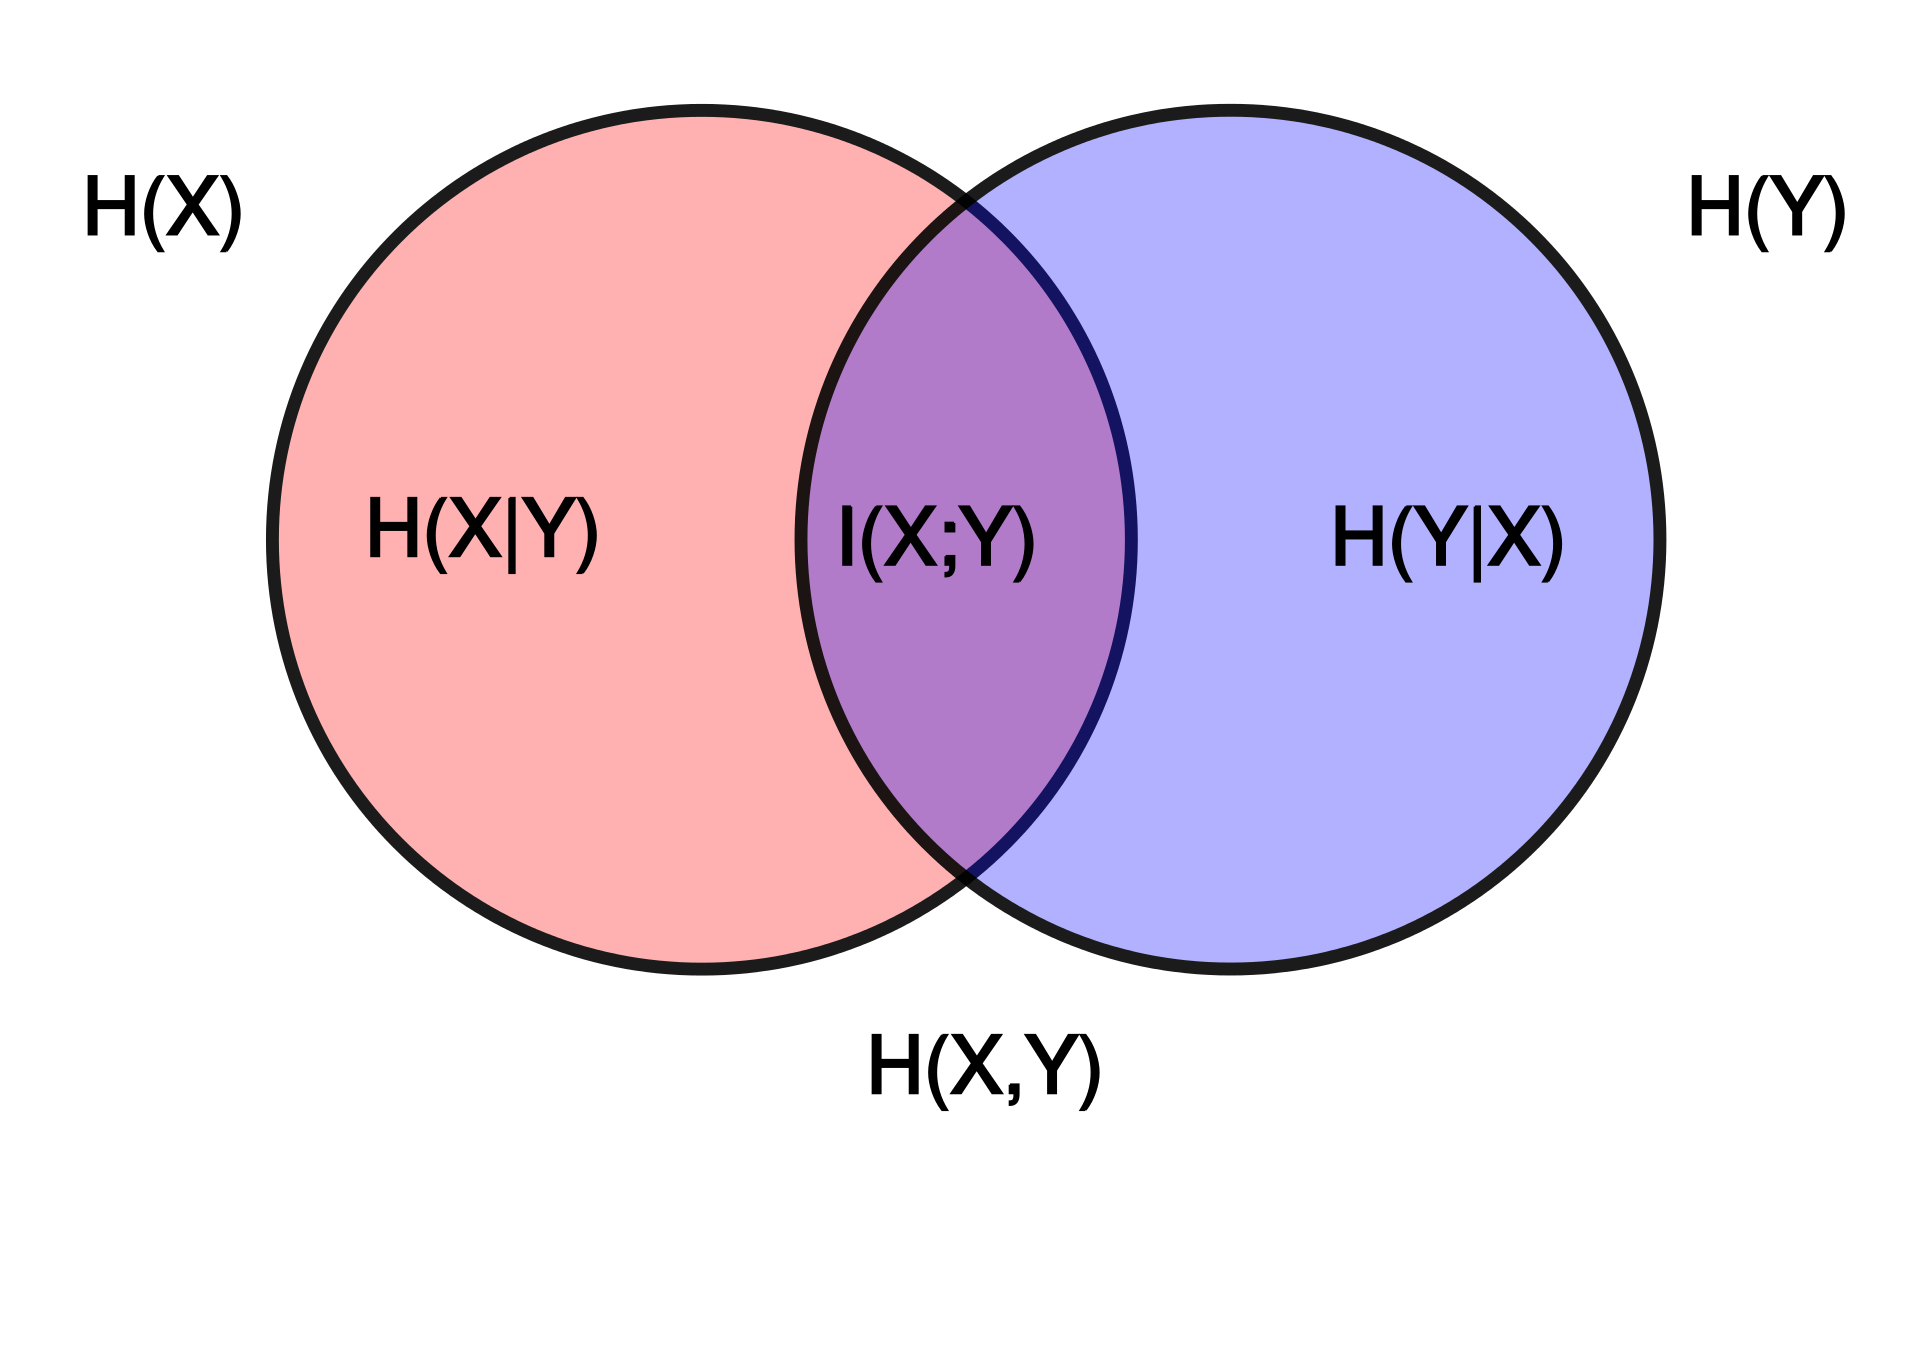
\includegraphics[width=0.7\textwidth]{includes/figures/defi_information_gain.png}
    \end{center}

    Information Gain wird von den Algorithmen \emph{ID3}, \emph{C4.5} und \emph{C5.0} genutzt.
\end{defi}

\begin{example}{Mutual Information}
    \begin{center}
        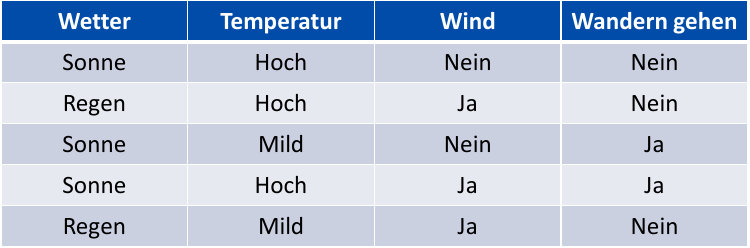
\includegraphics[width=0.6\textwidth]{includes/figures/example_information_gain.png}
    \end{center}

    % \begin{enumerate}[a)]
    %     \item Bestimmen Sie die Entropie für \enquote{Wandern gehen} (und geben Sie ihren Wert hier an).
    %     \item Bestimmen Sie die bedingten Entropien für \enquote{Wandern gehen} bezüglich der Features und geben Sie die Werte, die Sie erhalten haben, an.
    %     \item Bestimmen Sie den Information Gain für jedes Feature und geben sie die Werte hier an.
    % \end{enumerate}

    % \exampleseparator

    a) Bestimmen Sie die Entropie für \enquote{Wandern} (und geben Sie ihren Wert hier an).
    \[
        H(X) = - \sum_{k=1}^{C} p_k \log_2 p_k = - p_1 \log_2 p_1 - p_2 \log_2 p_2 = \frac{2}{5} \cdot \log_2 \frac{2}{5} - \frac{3}{5} \cdot \log_2 \frac{3}{5} \approx 0.97
    \]

    b) Bestimmen Sie die bedingten Entropien für \enquote{Wandern} bezüglich der Features und geben Sie die Werte, die Sie erhalten haben, an.
    \[
        H(Y \mid X) = - \sum_j p(x_j) \left( \sum_i p(y_i \mid x_j) \log_2 p(y_i \mid x_j) \right)
    \]

    Damit gilt:
    \[
        H(\text{Wandern} \mid \text{Wetter})
        = - \underbrace{\frac{3}{5} \left( \underbrace{\frac{2}{3} \log_2 \frac{2}{3}}_{\text{Wandern Ja}} + \underbrace{\frac{1}{3} \log_2 \frac{1}{3}}_{\text{Wandern Nein}} \right)}_{\text{Sonne}}
        - \underbrace{\frac{2}{5} \left( \underbrace{\frac{0}{2} \log_2 \frac{0}{2}}_{\text{Wandern Ja}} + \underbrace{\frac{2}{2} \log_2 \frac{2}{2}}_{\text{Wandern Nein}} \right)}_{\text{Regen}}
        \approx 0.55
    \]
    \[
        H(\text{Wandern} \mid \text{Temp.})
        = - \underbrace{\frac{3}{5} \left( \underbrace{\frac{1}{3} \log_2 \frac{1}{3}}_{\text{Wandern Ja}} + \underbrace{\frac{2}{3} \log_2 \frac{2}{3}}_{\text{Wandern Nein}} \right)}_{\text{Hoch}}
        - \underbrace{\frac{2}{5} \left( \underbrace{\frac{1}{2} \log_2 \frac{1}{2}}_{\text{Wandern Ja}} + \underbrace{\frac{1}{2} \log_2 \frac{1}{2}}_{\text{Wandern Nein}} \right)}_{\text{Mild}}
        \approx 0.95
    \]
    \[
        H(\text{Wandern} \mid \text{Wind})
        = - \underbrace{\frac{3}{5} \left( \underbrace{\frac{1}{3} \log_2 \frac{1}{3}}_{\text{Wandern Ja}} + \underbrace{\frac{2}{3} \log_2 \frac{2}{3}}_{\text{Wandern Nein}} \right)}_{\text{Wind Ja}}
        - \underbrace{\frac{2}{5} \left( \underbrace{\frac{1}{2} \log_2 \frac{1}{2}}_{\text{Wandern Ja}} + \underbrace{\frac{1}{2} \log_2 \frac{1}{2}}_{\text{Wandern Nein}} \right)}_{\text{Wind Nein}}
        \approx 0.95
    \]

    c) Bestimmen Sie die Mutual Information für jedes Feature und geben sie die Werte hier an.
    \[
        \text{IG}(Y, X) = H(Y) - H(Y \mid X)
    \]

    Damit gilt:
    \[
        \text{IG}(\text{Wandern}, \text{Wetter}) = H(\text{Wandern}) - H(\text{Wandern} \mid \text{Wetter})
        = 0.97 - 0.55 = 0.42
    \]
    \[
        \text{IG}(\text{Wandern}, \text{Temperatur}) = \ldots
        = 0.97 - 0.95 = 0.02
    \]
    \[
        \text{IG}(\text{Wandern}, \text{Wind}) = \ldots
        = 0.97 - 0.95 = 0.02
    \]
\end{example}

\begin{bonus}{Korrelation und Kausalität}
    Hohe Werte von Zusammenhangsmaßen können hindeuten auf kausale Zusammenhänge, diese aber nicht begründen.

    Kontrollierte Experimente können zur Entdeckung von kausalen Zusammenhängen genutzt werden.
    Typisch: Merkmal $X$ wird im Experiment verändert, und man beobachtet die daraus resultierenden oder nicht resultierenden Änderungen von Merkmal $Y$.

    Experimente lassen sich aber in vielen Fällen nicht realisieren.\footnote{Dieser Umstand begründet die Entwicklung von Maßen zur Charakterisierung der Richtung eines Zusammenhangs (z.B. \emph{Granger Causality})}
\end{bonus}

\subsection{Interpretationsfehler}

\begin{defi}{Scheinkausalität}
    Eine \emph{Scheinkausalität} ist eine Korrelation, die nicht mit einem kausalen Zusammenhang assoziiert ist.

    Es gibt drei Typen von Scheinkausalität:
    \begin{itemize}
        \item \emph{Common Driver}: Ein drittes Merkmal $X$, das mit $Y$ und $Z$ hochkorreliert ist, blieb in der Analyse zunächst unberücksichtigt.
              Wir beobachten also eine Scheinkorrelation zwischen $Y$ und $Z$.

              \begin{center}
                  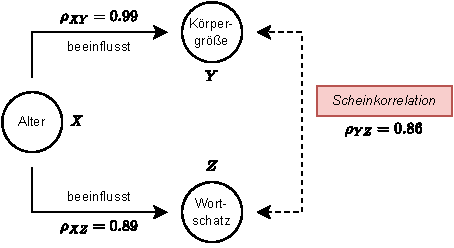
\includegraphics[width=.5\textwidth]{includes/figures/example_common_driver.pdf}
              \end{center}
        \item \emph{Indirekte Beziehung}:

              \begin{center}
                  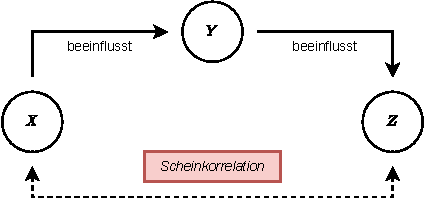
\includegraphics[width=.5\textwidth]{includes/figures/example_indirekte_beziehung.pdf}
              \end{center}
        \item \emph{Zufällige Korrelation}:

              \begin{center}
                  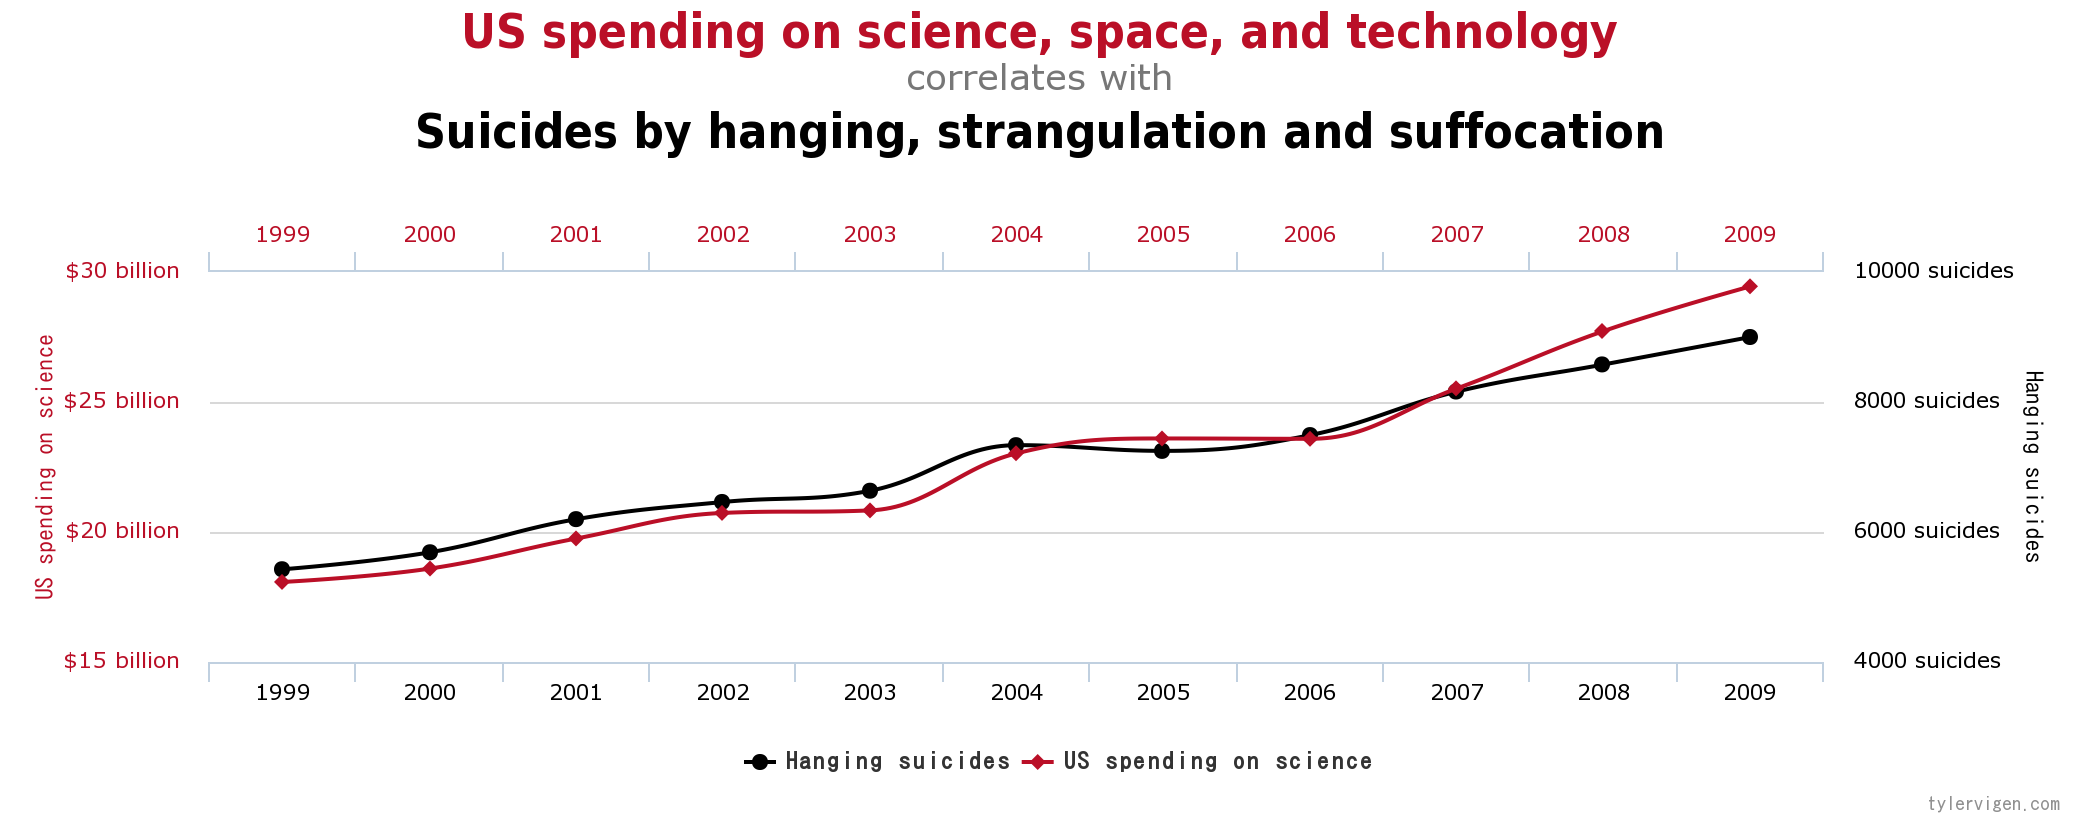
\includegraphics[width=.9\textwidth]{includes/figures/example_zufaellige_korrelation.png}
              \end{center}
    \end{itemize}


\end{defi}

\begin{defi}{Verdeckte Korrelation}
    Von einer \emph{verdeckten Korrelation} spricht man, wenn statistisch keinerlei Korrelation errechnet wurde, obwohl sachlich eindeutig Zusammenhänge vorliegen.

    Verdeckte Korrelation kann auftreten, wenn eine Population in Teilpopulationen zerfällt.
\end{defi}

\section{Dimensionsreduktionsverfahren}

\begin{defi}{Dimensionsreduktionstechnik}
    \emph{Dimensionsreduktionstechniken} reduzieren die Anzahl der Features (Merkmalen), die für Supervised oder Unsupervised Learning zur Verfügung stehen.
    \footnote{
        Oft mit dem Ziel, wenig Informationen dabei zu verlieren.
    }

    Ein Risiko besteht darin, dass prädikative Informationen für das Supervised Learning verloren gehen können.

    Chancen sind aber:
    \begin{itemize}
        \item Schnellere Berechnungen durch Weglassen irrelevanter Informationen
        \item Ermöglichung von Visualisierung der Daten (und damit der Gewinnung von Einsichten) im Rahmen einer explorativen Analyse (Data Science)
        \item Ermöglichung besserer Generalisierung von Lernmodellen durch Entgegenwirken der Curse of Dimensionality (Fluch der Dimensionalität)
    \end{itemize}
\end{defi}

\begin{bonus}{Curse of Dimensionality}
    Der \emph{Curse of Dimensionality} im Kontext des Machine Learnings das Phänomen, nach dem das Volumen des Feature-Raumes dramatisch zunimmt mit der Anzahl der Dimensionen, so dass die $N$ Datenpunkte (der Trainingsmenge) nur noch spärlich (sparse) im Raum liegen.

    Typische Folgen sind:
    \begin{itemize}
        \item Overfitting-Tendenz steigt
        \item Rechenzeit steigt
        \item Lernmodelle generalisieren schlecht
    \end{itemize}

    Wenn Daten nur noch spärlich den Feature-Raum ausfüllen, dann wird es schwierig, Modelle an die Daten anzupassen, die den Raum adäquat beschreiben
\end{bonus}

\subsection{Principal Component Analysis (PCA)}

\begin{defi}{Principal Component Analysis}
    Die \emph{Hauptkomponentenzerlegung} (\emph{Principal Component Analysis}, PCA) zählt zu den bekanntesten Dimensionsreduktionsverfahren.

    PCA findet neue Achsen (Komponenten) für die Daten, so dass die Daten bezüglich dieser Achsen eine \emph{möglichst große Varianz} aufweisen.

    Achsen, bezüglich derer die Daten kaum (oder keine) Varianz anweisen, können später weggelassen werden (Dimensionsreduktion).

    Neue Achsen werden durch orthogonale Transformation erzeugt, d.h. Vektorlängen und Winkel bleiben erhalten.
    \footnote{
        Präziser: das innere Produkt bleibt erhalten.
    }

    Sei die \emph{Kovarianzmatrix} $S$ gegeben mit:
    \[
        S = \frac{1}{N} \sum_{n=1}^N (\mathbf{x}_n - \conj{\mathbf{x}_n}) (\mathbf{x}_n - \conj{\mathbf{x}_n})^T
    \]

    Dann gilt:
    \begin{itemize}
        \item Eigenwertzerlegung der Kovarianzmatrix $S$ liefert Eigenwerte $\lambda_j$ und -vektoren $\mathbf{u}_j$.
        \item Wir sortieren nach Größe der Eigenwerte und erhalten die Richtungen der PCA über die zu den Eigenwerten assoziierten Eigenvektoren von S.
    \end{itemize}

    PCA kann als Transformation interpretiert werden, die die Achsen des Koordinatensystems so rotiert, dass die Varianz der Projektion der Daten auf der ersten Achse maximiert wird.

    Der Mittelwert der Daten beeinflusst die PCA-Koordinaten:
    \begin{itemize}
        \item Daten mit Schwerpunkt (Mittelwert), der nicht dem Koordinatenursprung entspricht, haben nach PCA-Transformation in den neuen Koordinaten typischerweise Offsets, die meist nicht gut interpretierbar sind.
        \item PCA-Richtungen ändern sich nicht unter Änderung des Schwerpunkts der Daten. Grund: Kovarianzmatrix ist invariant\footnote{Die Kovarianzmatrix verändert sich nicht.} unter Transformation der Mittelwerte.
        \item Manche Software-Implementierungen nutzen für die PCA nicht die Kovarianzmatrix. Dort kann die PCA von den Mittelwerten der Daten abhängen.
    \end{itemize}

    \emph{Jedes Merkmal sollte auf den Mittelwert $0$ zentriert werden}:
    \[
        \tilde{x}_i = x_i - \conj{x}, \quad \forall i
    \]

    Die Skalierung der Daten beeinflusst PCA:
    \begin{itemize}
        \item Die Skalen, in der ein Merkmal angegeben wird beeinflusst die Varianz dieses Merkmals.
        \item Die Ergebnisse der PCA ist abhängig von den Varianzen der Merkmale.
    \end{itemize}

    \emph{Jedes Merkmal sollte auf eine Varianz von $1$ skaliert werden, damit die Ergebnisse der PCA nicht von der (eventuell) willkürlichen Wahl der Skalen der Merkmale abhängig ist}:
    \[
        \tilde{x}_i = \frac{x_i}{\sigma}, \quad \forall i
    \]
\end{defi}

\begin{bonus}{Standardisierung}
    \emph{Standardisierung} bzw. \emph{z-scoring} beschreibt die Transformation eines Merkmals $X$, so dass es Mittelwert $0$ und Varianz $1$ aufweist.
    Das Merkmal wird also \emph{zentriert} und \emph{skaliert}.

    Sei $\conj{X}$ der Mittelwert und $\sigma$ die Standardabweichung von $X$.

    Das \emph{standardisierte Merkmal} bzw. der \emph{z-score} $Z$ wird erzeugt durch:
    \[
        Z = \frac{X - \conj{X}}{\sigma}
    \]

    In der Praxis liegen sind Daten oft in Matrizen organisiert, in denen jede Spalte einem Merkmal entsprechen.
    In diesem Fall standardisiert man jedes Merkmal, indem jede Spalte separat auf Mittelwert 0 und Varianz 1 transformiert wird.
\end{bonus}

\begin{defi}{Proportion of Variance Explained}
    \emph{Proportion of Variance Explained (PVE)} beschreibt den Bruchteil der Gesamtvarianz der Merkmale, die über die PCA-Komponenten repräsentiert wird.

    Die Varianz der $j$-ten Komponente ist:\footnote{Entspricht also dem jeweiligen Eigenwert.}
    \[
        \Var(Z_j) = \Var(\mathbf{u}_j^T \mathbf{x}) = \mathbf{u}_j^T \mathbf{S} \mathbf{u}_j = \mathbf{u}_j^T \lambda_j \mathbf{u}_j = \lambda_j
    \]

    Die Gesamtvarianz über alle Merkmale ist dann:
    \[
        \Var_\text{total} = \sum_{j=1}^D \Var(Z_j) = \sum_{j=1}^D \lambda_j
    \]

    Dann ist die $\PVE(j)$ der $j$-ten PCA-Komponente definiert als:
    \[
        \PVE(j) = \frac{\Var(Z_j)}{\Var_\text{total}} = \frac{\lambda_j}{\sum_{j=1}^D \lambda_j}
    \]
\end{defi}

\subsection{Multidimensional Scaling (MDS)}

\begin{defi}{Multidimensional Scaling}
    \emph{Multidimensional Scaling (MDS)} ist eine Familie von Verfahren für die Visualisierung von Punkten (durch Finden geeigneter Koordinaten) sowie zur Dimensionsreduktion von Daten.

    Gegeben seien die paarweisen Distanzen zwischen $N$ Objekten, in Form einer $N \times N$-Matrix der paarweisen euklidischen Distanzen:
    \[
        D = (d_{rs})
    \]

    Gesucht ist dann die Datenmatrix $X$, die die Koordinaten (Features) für jedes der $N$ Objekte enthält, so dass die Objekte in diesen Koordinaten die paarweisen euklidischen Distanzen $D = (d_{rs})$ aufweisen.

    Mit diesen Koordinaten lassen sich die Objekte z. B. visualisieren.

    Die Lösung ist dabei nicht eindeutig, da die Distanzen invariant sind unter:
    \begin{itemize}
        \item orthogonalen Transformationen (Rotation, Spiegelung)
        \item Koordinatenverschiebung
    \end{itemize}

    Das Vorgehen ist wie folgt:
    \begin{enumerate}
        \item Ermitteln der Distanzmatrix $D$ (quadrierte euklidische Distanzen)
        \item Ermitteln der Matrix $B$ durch Zentrierung der Matrix $D$:
              \[
                  B = - \frac{1}{2} HDH, \quad H = I - \frac{1}{N} \mathbf{1} \mathbf{1}^T
              \]
        \item Durchführen einer Eigenwertzerlegung von $B$
        \item Mithilfe der Eigenwerte und -vektoren Erzeugen von Datenmatrix $X$:
              \[
                  X = \begin{bmatrix}
                      \sqrt{\lambda_1} \mathbf{v}_1 & \sqrt{\lambda_2} \mathbf{v}_2 & \cdots & \sqrt{\lambda_P} \mathbf{v}_P
                  \end{bmatrix}
              \]
              wobei die Eigenwerte und assoziierten Eigenvektoren der Größe nach absteigend sortiert wurden.
    \end{enumerate}
\end{defi}

\begin{defi}{Proportion of Distance Matrix Explained}
    \emph{Proportion of Distance Matrix Explained} (PDME) funktionert analog der Proportion of Variance Explained (PVE) für die PCA.

    Dann ist die $\PDME(j)$ der $j$-ten PCA-Komponente definiert als:
    \[
        \PDME(j) = \frac{\lambda_j}{\sum_{i=1}^{N} |\lambda_i|}, \quad \forall j \; \text{mit} \; \lambda_j \geq 0
    \]
\end{defi}

\begin{bonus}{MDA vs. PCA}
    Wenn:
    \begin{itemize}
        \item Datenmatrix $X$ zentriert ist (d.h. Mittelwertvektor ist 0)
        \item Distanzmatrix $D$ aus euklidischen Distanzen besteht
    \end{itemize}
    dann sind MDS-Koordinaten und PCA-Koordinaten der Daten identisch.

    Die Matrizen $X^TX$ (PCA) und $XX^T$ (MDS) haben dann gemeinsame Eigenwerte und ihre Eigenvektoren sind proportional zueinander.

    Unterschiede sind aber:
    \begin{itemize}
        \item Ausgangssituation (bei MDS ist Distanzmatrix bekannt, Koordinaten aber nicht)
        \item MDS ist Ausgangspunkt für verschiedene Verfahren, z. B. Isomap
        \item PCA nicht nutzbar bei nichtlinearen Strukturen
    \end{itemize}
\end{bonus}

\begin{defi}{Isomap}
    \emph{Isomap} nutzt Multidimensional Scaling (MDS), aber errechnet die Distanzmatrix $D$ aus einem Nächste-Nachbarn Graphen der Datenpunkte.

    Der Algorithmus funktioniert wie folgt:
    \begin{enumerate}
        \item Ermittle Nachbarschaftsgraph mit euklidischen Distanzen:
              \begin{enumerate}
                  \item Verbinde einen Punkt mit seinen $k$-nächsten Nachbarn
                  \item Verbinde einen Punkt mit allen Nachbarn innerhalb eines Epsilonballs
              \end{enumerate}
        \item Distanzmatrix $D$:
              \begin{enumerate}
                  \item Ermittle paarweise Distanzen zwischen Punkten auf dem Graph
                  \item Quadriere diese Distanzen
              \end{enumerate}
        \item Wende Multidimensional Scaling auf Distanzmatrix $D$ an und erhalte Datenmatrix $X$
    \end{enumerate}
\end{defi}
\section{Clustering}

\begin{defi}{Clusteranalyse}
    Die \emph{Clusteranalyse} findet Gruppen (\emph{Cluster}) ähnlicher Datenpunkte, ohne dass Labels vorliegen müssen.

    \emph{Clustering} ist also Partitionierung (Einteilung) der Datenpunkte in Gruppen.

    Viele Clusteranalyseverfahren existieren und unterscheiden sich:
    \begin{itemize}
        \item in der Definition von Ähnlichkeit,
        \item in der Definition von Gruppen (Clustern),
        \item im algorithmischen Vorgehen.
    \end{itemize}

    Es gilt:
    \begin{itemize}
        \item Clusteranalyseverfahren finden immer Cluster in den Daten.
        \item Verschiedene Verfahren liefern verschiedene Cluster für dieselben Daten.
        \item Cluster-Verfahren interpretieren die Daten hinsichtlich der den Verfahren (teils implizit) zugrundeliegenden Annahmen.
        \item Wie Clusterings bewertet werden können (also z.B. als sinnvoll bzw. nicht sinnvoll eingestuft werden können), ist aktuelles und im Allgemeinen ungelöstes Forschungsproblem.
    \end{itemize}
\end{defi}

\begin{defi}{K-Means Clustering}
    Seien $C_1, \ldots, C_K$ die Mengen der Indizes der Datenpunkte jedes Clusters.

    Die Mengen sollen zwei Eigenschaften erfüllen:
    \begin{enumerate}
        \item Jeder Datenpunkt gehört zu mindestens einem Cluster:
              \[
                  C_1 \cup C_2 \cup \ldots \cup C_K = \{ 1, \ldots, N \}
              \]
        \item Die Cluster überlappen nicht.
              Jeder Datenpunkt gehört nicht mals als einem Cluster an.
              \[
                  C_k \cap C_{k'} = \emptyset, \quad \forall k \neq k'
              \]
    \end{enumerate}

    Wenn der $i$-te Datenpunkt zum $k$-ten Cluster gehört, dann gilt: $i \in C_k$.

    Die Hauptidee hinter \emph{K-Means Clustering} ist, dass das Clustering gut ist, wenn die \emph{Intra-Cluster-Variation} minimiert wird.

    Bezeichne $W(C_k)$ die Intra-Cluster-Variation des $k$-ten Clusters.
    Sie ist definiert als Summe der quadratischen euklidischen Distanzen zwischen allen Datenpunkten eines Clusters:
    \[
        W(C_k) = \frac{1}{\abs{C_k}} \sum_{i, i' \in C_k} \sum_{j=1}^p (x_{ij} - x'_{i'j})^2
    \]

    Es ist die Summe der Intra-Cluster-Variationen zu minimieren:
    \[
        \min_{C_1, \ldots, C_k} \, \left\{ \sum_{k=1}^K W(C)_k \right\} = \min_{C_1, \ldots, C_k} \, \left\{ \sum_{k=1}^K \frac{1}{\abs{C_k}} \sum_{i, i' \in C_k} \sum_{j=1}^p (x_{ij} - x'_{i'j})^2 \right\}
    \]

    Das Vorgehen ist also wie folgt:
    \begin{enumerate}
        \item Weise allen Datenpunkten zufällige Clusterzugehörigkeiten $1, \ldots, K$ zu.
        \item Iteriere, bis die Cluster sich nicht mehr ändern:
              \begin{enumerate}
                  \item Für jeden der K Cluster, berechne den \emph{geometrischen Schwerpunkt} (\emph{centroid}).

                        Der Schwerpunkt ist der Featurevektor, der sich aus der Mittelung aller Featurevektoren der dem Cluster zugehörigen Datenpunkte ergibt.
                  \item Weise jedem Datenpunkt dem Cluster zu, dessen Schwerpunkt dem Datenpunkt am nächsten liegt (im euklidischem Sinne).
              \end{enumerate}
    \end{enumerate}

    Es gilt:
    \begin{itemize}
        \item K-Means Clustering hängt ab von der zufälligen Anfangsinitialisierung der Clusterzugehörigkeiten.

              Der 1. Schritt findet lokale Minima unserer Optimierungsfunktion, nicht notwendigerweise das globale Minimum.
        \item Clusteranzahl K muss zu Beginn festgelegt werden.
              Verschiedene Werte für $K$ können ganz unterschiedliche Cluster liefern.
        \item Keine Möglichkeit, Ausreißer in den Daten zu erkennen und getrennt zu behandeln.
    \end{itemize}

    Eine Empfehlung ist, K-Means mehrfach mit zufälligen initialen Clusterzugehörigkeiten zu versuchen und dann das Ergebnis mit dem kleinsten Wert für die summierte Intra-Cluster-Variation zu wählen.
\end{defi}

\begin{defi}{Hierarchische Clusteranalyse}
    Die \emph{Hierarchische Clusteranalyse (HCA)} erzeugt eine Menge verschiedener Aufteilung der Daten in Cluster (\emph{Partitionierungen}), aus denen eine Partition (\emph{Clustering}) ausgewählt wird.

    Das Konzept ist der Aufbau eines \emph{Dendrogramms}; ein Dendrogramm ist ein Diagramm, das einen Baum repräsentiert.\footnote{Bäume können von den Blättern hin zur Wurzel (\emph{agglomeratives Clustern}, Bottom-Up), oder von der Wurzel hin zu den Blättern (\emph{divisives Clustern}, Top-Down) aufgebaut werden. In der Vorlesung wird der Bottom-Up-Ansatz behandelt.}

    Jeder Datenpunkt entspricht einem Blatt im Dendrogramm.

    Je höher im Baum gewandert wird, desto mehr Blätter werden zu Zweigen verbunden.

    Je früher (weiter unten) Zweige bzw. Blätter verbunden werden, desto ähnlicher sind die entsprechenden Datenpunkte.

    Für jedes Paar von Datenpunkten zeigt die Höhe (y-Achse) der Verbindung der beiden ihre Unterschiedlichkeit (\emph{dissimilarity}) an.

    Der Algorithmus ist wie folgt:
    \begin{enumerate}
        \item Betrachte alle $N$ Datenpunkte und interpretiere sie als $N$ separate Cluster.
        \item Wähle ein Maß für die Unterschiedlichkeit (\emph{dissimilarity measure} (Datenpunkte) bzw. \emph{Linkage} (Cluster)) aus:
              \begin{itemize}
                  \item Für Datenpunkte: oft \emph{euklidische Distanz}
                  \item Für Cluster: \emph{complete, single, average Linkage}
              \end{itemize}
        \item Für $i = N, N-1, \ldots, 2$:
              \begin{enumerate}
                  \item Bestimme die paarweisen Unterschiedlichkeiten für alle Cluster und fusioniere das Clusterpaar, das sich am ähnlichsten ist, zu einem neuen Cluster.

                        Die Unterschiedlichkeit zwischen den beiden soeben fusionierten Clustern entspricht der Höhe im Dendrogramm, in der der Zusammenschluss stattfindet.
                  \item Berechne die neuen paarweisen Unterschiedlichkeiten zwischen den $i-1$ übrig gebliebenen Clustern.
              \end{enumerate}
    \end{enumerate}
\end{defi}

\begin{defi}{Complete Linkage}
    \emph{Complete Linkage} entspricht der \emph{maximalen} Inter-Cluster-Unterschiedlichkeit.

    Vorgehen:
    \begin{enumerate}
        \item Alle paarweisen Unterschiedlichkeiten zwischen Punkten aus dem ersten und Punkten aus dem zweiten Cluster bestimmen.
        \item Unterschiedlichkeit zwischen beiden Clustern entspricht der \emph{größten Unterschiedlichkeit}.
    \end{enumerate}

    \begin{center}
        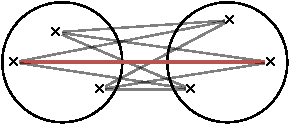
\includegraphics[width=0.55\textwidth]{includes/figures/defi_complete_linkage.pdf}
    \end{center}
\end{defi}

\begin{defi}{Single Linkage}
    \emph{Single Linkage} entspricht der \emph{minimalen} Inter-Cluster-Unterschiedlichkeit.

    Vorgehen:
    \begin{enumerate}
        \item Alle paarweisen Unterschiedlichkeiten zwischen Punkten aus dem ersten und Punkten aus dem zweiten Cluster bestimmen.
        \item Unterschiedlichkeit zwischen beiden Clustern entspricht der \emph{kleinsten Unterschiedlichkeit}.
    \end{enumerate}

    Single Linkage liefert oft unausgewogene Cluster.
    \begin{center}
        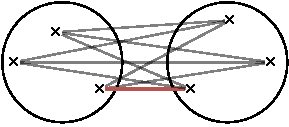
\includegraphics[width=0.55\textwidth]{includes/figures/defi_single_linkage.pdf}
    \end{center}
\end{defi}

\begin{defi}{Average Linkage}
    \emph{Average Linkage} entspricht der \emph{mittleren} Inter-Cluster-Unterschiedlichkeit.

    Vorgehen:
    \begin{enumerate}
        \item Alle paarweisen Unterschiedlichkeiten zwischen Punkten aus dem ersten und Punkten aus dem zweiten Cluster bestimmen.
        \item Unterschiedlichkeit zwischen beiden Clustern entspricht dem \emph{Mittelwert der Unterschiedlichkeit}.
    \end{enumerate}

    \begin{center}
        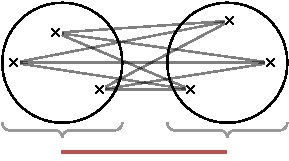
\includegraphics[width=0.55\textwidth]{includes/figures/defi_average_linkage.pdf}
    \end{center}
\end{defi}

\begin{bonus}{K-Means vs Hierarchisches Clustern}
    Clustering Verfahren interpretieren die Daten mit den ihnen impliziten und expliziten Annahmen, wie Cluster zu definieren sind.

    \emph{Hierarchisches Clustern}: Annahme, dass Cluster hierarchisch organisiert sind (d.h. große Cluster setzen sich aus kleineren Clustern zusammen).

    \emph{K-Means Clustering}: Annahme, dass Cluster sphärische Objekte im Feature-Space sind und ungefähr gleich viele Datenpunkte enthalten.
\end{bonus}

\begin{bonus}{Clusteranalyse Hinweise}
    Worauf man achten sollte:
    \begin{enumerate}
        \item Wahl des Unterschiedlichkeitsmaßes (dissimilarity measure)
        \item Vorverarbeitung der Daten
              \begin{itemize}
                  \item Untersuchung, welche Auswirkungen eine Skalierung der Features in Kombination mit der Wahl des Unterschiedlichkeitsmaß (dissimilarity measure) auf Cluster-Ergebnisse hat.
              \end{itemize}
        \item Wahl der Clusteranzahl (oder anderer freier Parameter)
              \begin{itemize}
                  \item Untersuchung, welche Auswirkungen Ihre Wahl einer Clusteranzahl auf Cluster-Ergebnisse hat.
              \end{itemize}
        \item Interpretation der Ergebnisse
              \begin{itemize}
                  \item Cluster-Analyse als Startpunkt einer Untersuchung der Daten, nicht als Endpunkt einer Analyse.
              \end{itemize}
    \end{enumerate}
\end{bonus}
\section{Clustervalidierungsverfahren}

\begin{defi}{Clustervalidierungsverfahren}
    \emph{Clustervalidierungsverfahren} bewerten die Qualität von Clusterings (Partitionen) und ermöglichen so das Einstellen von Hyperparametern\footnote{Beispiel: Anzahl $K$ der Cluster bei K-Means}.

    Man unterscheidet zwischen drei Arten:
    \begin{enumerate}
        \item \emph{Tests auf Abwesenheit von Clusterstruktur}
              \begin{itemize}
                  \item häufig in Forschungskontexten, selten in der Praxis
                  \item Tests gegen typische Nullhypothesen
                        \begin{itemize}
                            \item Daten liegen zufällig verteilt im Merkmalsraum (\emph{Uniformitätshypothese})
                            \item Daten wurden aus unimodaler Verteilung gezogen (\emph{Unimodale Nullhypothese})
                        \end{itemize}
              \end{itemize}
        \item \emph{Externe Clustervalidierung}
              \begin{itemize}
                  \item Kriterien, die auf externen Informationen über die wahre Clusterzugehörigkeiten basieren
              \end{itemize}
        \item \emph{Interne Clustervalidierung}
              \begin{itemize}
                  \item Kriterien, die allein auf den Daten basieren
              \end{itemize}
    \end{enumerate}
\end{defi}

\subsection{Externe Clustervalidierung}

\begin{defi}{Purity}
    Die \emph{Purity} misst die Reinheit von Clustern.

    Dabei sind:
    \begin{itemize}
        \item $C_1, \ldots, C_K$ Mengen der \emph{Indizes} der Datenpunkte jedes Clusters.
        \item $T_1, \ldots, T_K$ Mengen der \emph{Indizes} der Datenpunkte der \emph{wahren} Cluster gemäß der externen Information (\emph{ground truth})
        \item $N_i = |C_i|$ Anzahl der Datenpunkte in Cluster $i$
    \end{itemize}

    Dann ist die Purity des Clusters $i$:
    \[
        \purity_i = \frac{1}{N_i} \cdot \max_{j=1}^{K} |C_i \cap T_j|
    \]

    Die Purity des Clusters $i$ wird also 1, wenn es nur Punkte eines wahren Clusters in der Partition $T$ enthält.

    Die gesamte Purity ist:
    \[
        \purity = \sum_{i=1}^{K} \frac{N_i}{N} \purity_i
    \]

    Die Purity der Partitionierung wird also 1, wenn alle Cluster $i$ nur Punkte eines wahren Clusters enthalten.
\end{defi}

\begin{bonus}{Mutual Information}
    \emph{Mutual Information} ist ebenfalls ein externes Clustervalidierungsverfahren.

    Hierbei gilt mit
    \begin{itemize}
        \item $p_{ij}$ Wahrscheinlichkeit, dass ein Datenpunkt aus Cluster $i$ zur Partition $j$ aus $T$ gehört
        \item $p_{C_i}$: Wahrscheinlichkeit für Cluster $C_i$
        \item $p_{T_i}$: Wahrscheinlichkeit für Cluster $T_i$
    \end{itemize}
    \[
        \IG(C, T) = \sum_{i, j} p_{ij} \log_2 \left(\frac{p_{ij}}{p_{C_i} p_{T_j}}\right)
    \]
\end{bonus}

\subsection{Interne Clustervalidierung}

\begin{defi}{Silhouettenindex}
    Seien $C_A$, $C_B$, $C_C$ Mengen, die die Indizes der Datenpunkte in den Clustern $A$, $B$ und $C$ enthalten.

    Sei $i \in C_A$ ein Datenpunkt des Clusters $A$.

    Sei $d_{ij}$ die (euklidische) Distanz zwischen den Punkten $i$ und $j$.

    Dann ist die \emph{Kohäsion}, die mittlere Distanz zwischen $i$ und allen Punkten in Cluster $A$:\footnote{$-1$ bzw. $j \neq i$, da wir nicht über $d_{ii}$ summieren.}
    \[
        \koh(i) := \frac{1}{|C_A| - 1} \sum_{j \in C_A, j \neq i} d_{ij}
    \]

    Und die \emph{Seperation}, die mittlere Distanz zwischen $i$ und allen Punkten im benachbarten Cluster (hier $X = B$):
    \[
        \sep(i) := \min_{X \neq A} \frac{1}{|C_X|} \sum_{j \in C_X} d_{ij}
    \]

    $i$ ist gut geclustert, wenn:
    \begin{itemize}
        \item Kohäsion gering
        \item Seperation hoch
    \end{itemize}

    Der \emph{Silhouettenindex} ist dann definiert als:
    \[
        s(i) = \begin{cases}
            1 - \frac{\koh(i)}{\sep(i)}, & \text{falls} \ \koh(i) < \sep(i) \\
            0,                           & \text{falls} \ \koh(i) = \sep(i) \\
            \frac{\sep(i)}{\koh(i)} - 1, & \text{falls} \ \koh(i) > \sep(i)
        \end{cases}
        = \frac{\sep(i) - \koh(i)}{\max \{\koh(i), \sep(i)\}}
    \]

    Um ein Cluster zu bewerten, verwendet man die \emph{Average Silhouette Width}:
    \[
        \conj{s}_X = \frac{1}{|C_X|} \sum_{i \in C_X} s(i)
    \]

    Um das komplette Clustering zu bewerten, verwendet man den \emph{Silhouette Score}:
    \[
        \conj{s} = \frac{1}{N} \sum_{i = 1}^{N} s(i)
    \]
\end{defi}

\begin{defi}{Silhouettenplot}
    \emph{Silhouettenplots} stellen Silhouettenindizes nach Cluster gruppiert und in absteigender Größe dar.

    Sie erlauben eine visuelle Einschätzung der Clusterqualität.

    Silhouettenplots interpretieren Cluster als kompakte, sphärische Objekte.
    Dies ist aber nicht notwendigerweise der Fall.
\end{defi}

\begin{example}{Silhouettenplot}
    \centering
    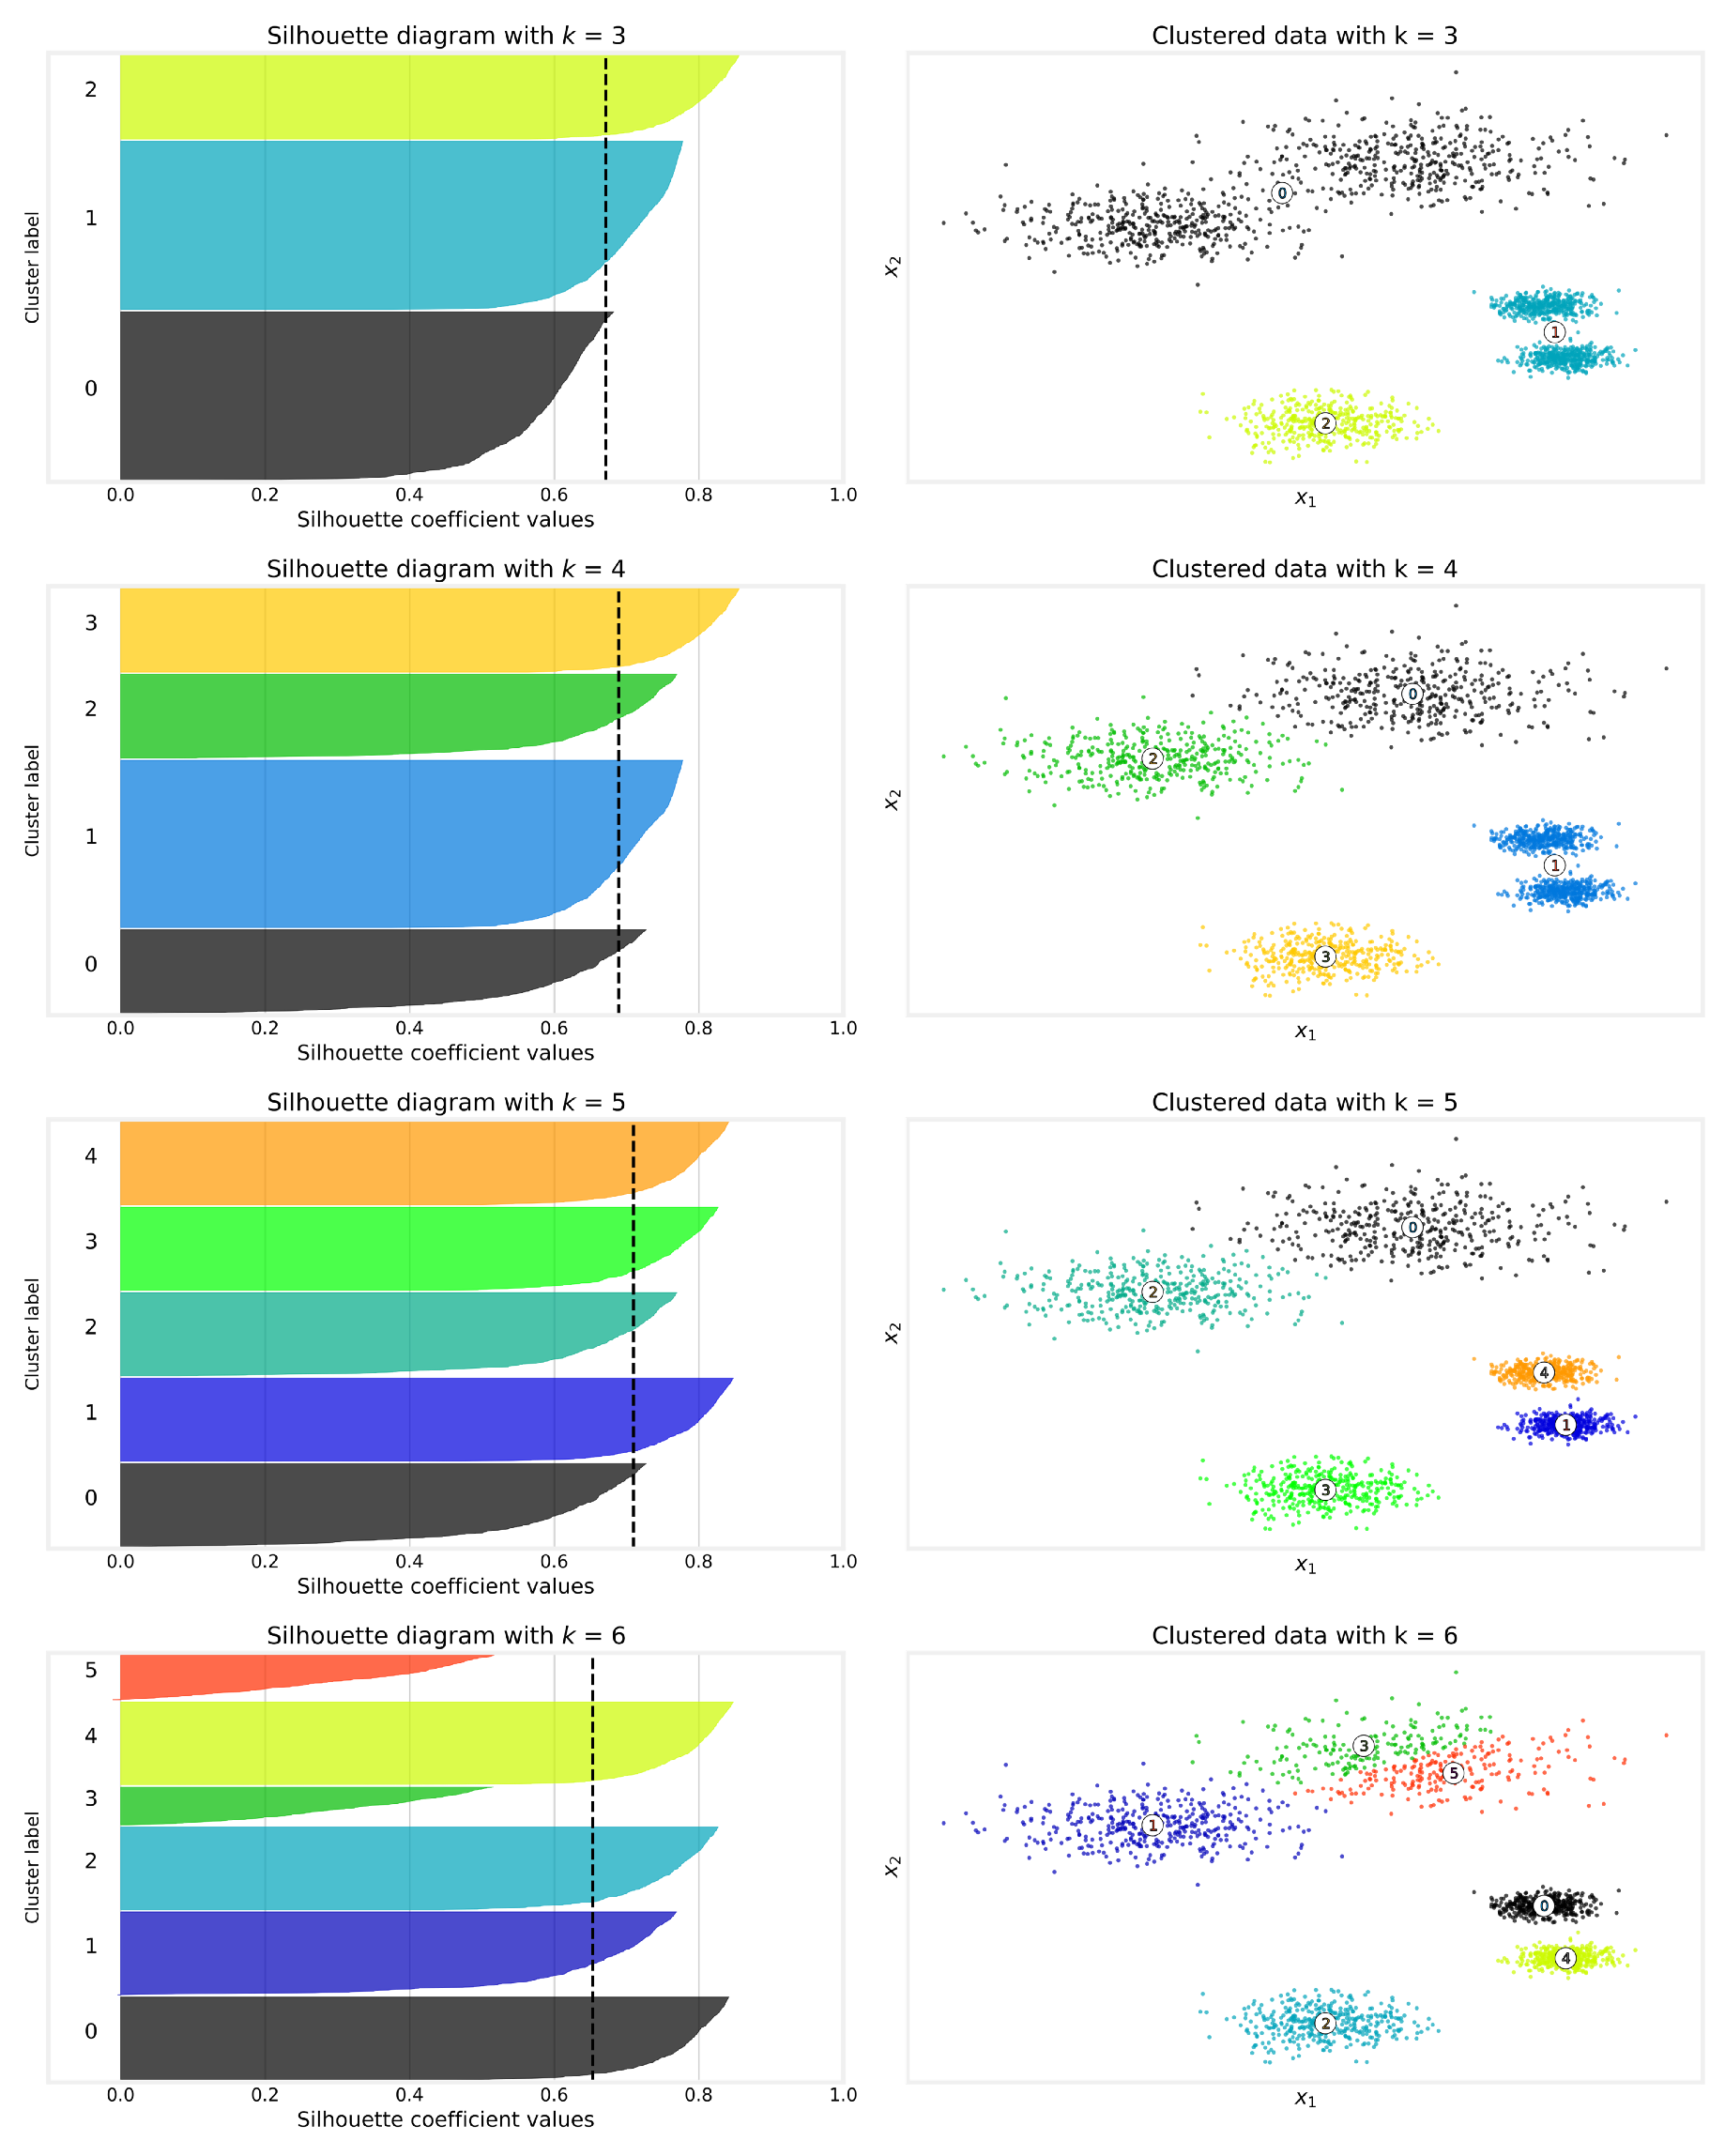
\includegraphics[width=\textwidth]{includes/figures/example_silhouette_plot.png}
\end{example}

\begin{defi}{Prediction Strength}
    Die Idee der \emph{Prediction Strength} ist, dass die  Clusterqualität hoch ist, wenn Clusterzugehörigkeiten auf anderer Realisation der Daten zuverlässig vorhergesagt werden können.

    Das Verfahren ist wie folgt:
    \begin{enumerate}
        \item Zufälliges Aufteilen der Daten $\mathcal{D}$ in zwei Mengen: Trainings- und Validierungsset $\mathcal{D}_\text{train}$ und Validierungsset $\mathcal{D}_\text{val}$.
        \item Clustern der Trainingsdaten und Validierungsdaten separat mit denselben gewählten Parametern.
        \item Ermitteln der Clusterzugehörigkeiten für alle Daten in $\mathcal{D}_\text{val}$ gemäß des Clusterings in $\mathcal{D}_\text{train}$.
        \item Bestimmung des Bruchteils $p$ aller Paare von Datenpunkten in $\mathcal{D}_\text{val}$, die sich auch im selben Cluster in $\mathcal{D}_\text{train}$ befinden würden.
              Der kleinste Wert $p$ über aller Cluster heißt \emph{Prediction Strength}.
    \end{enumerate}

    Sei $M$ eine $N_{\text{val}} \times N_{\text{val}}$-Matrix (\emph{Ko-Mitgliedsschaftsmatrix}) mit
    \[
        M_{i, i'} :=
        \begin{cases}
            1, & \exists k: (i, i') \in R_{C_k} \\
            0, & \text{sonst}
        \end{cases}
    \]
    d. h. ein Matrixeintrag ist 1, wenn die jeweiligen zwei Datenpunkte aus dem Validierungsset zur selben Region eines Clusters $k$ im Trainingset gehören.

    Formal ist die Prediction Strength folgendermaßen definiert:\footnote{$R_{C_k}$ ist die Region des Clusters $k$ im Trainingsset.}
    \[
        \ps(K) = \min_{j = 1, \ldots, K} \frac{1}{|A_j| (|A_j| - 1)} \sum_{i, i' \in A_i, i \neq i'} M_{ii'}
    \]
\end{defi}
\section{Feature Engineering}

\begin{defi}{Feature Engineering}
    \emph{Feature Engineering} ist der Prozess, mithilfe von Domänenwissen Merkmale aus Rohdaten zu erzeugen, um die datengetriebene Modellierung (und damit Vorhersagen) zu ermöglichen.

    Feature Engineering vermittelt zwischen Rohdaten und Modellen.

    Feature Engineering ist
    \begin{itemize}
        \item meist zeitaufwändig
        \item oft entscheidend für den Erfolg eines Machine Learning Projektes
        \item domänenspezifisch
    \end{itemize}

    Typisches Vorgehen (eines Data Scientist) beim Feature Engineering:
    \begin{enumerate}
        \item Klassische Methoden der Explorativen Analyse (EDA) werden genutzt
        \item Domänenexperten aufsuchen und über Daten und ihre wichtigsten Eigenschaften befragen
        \item Selbst zum Domänenexperten für bestimmte Datenarten werden (typischerweise während der Berufsausübung oder wissenschaftlichen Ausbildung)
    \end{enumerate}
\end{defi}

\begin{defi}{Klassifikation}
    Bei der (binären) \emph{Klassifikation} unterscheidet ein Modell zwischen zwei Klassen.

    Das einfachste Modell dabei ist eine Schwellwert-basierte Klassifikation.

    Bei der \emph{Multiklassen-Klassifikation} unterscheidet ein modell zwischen mehr als zwei Klassen.
\end{defi}

\begin{defi}{Accuracy}
    Die \emph{Accuracy} ist ein Maß, um die Genauigkeit eines Klassifikators zu messen.

    Sie ist die Anzahl der richtig klassifizierten Datenpunkte dividiert durch Gesamtzahl aller Datenpunkte:
    \[
        \ACC = \frac{\TP + \TN}{\TP + \TN + \FN + \FP}
    \]
    mit:
    \begin{itemize}
        \item $\TP$: True Positive (Richtige Klassifikation)
        \item $\TN$: True Negative (Richtige Klassifikation)
        \item $\FP$: False Positive (Falsche Klassifikation)
        \item $\FN$: False Negative (Falsche Klassifikation)
    \end{itemize}

    Nachteile:
    \begin{itemize}
        \item anfällig gegenüber ungleich großen Klassen (\emph{class imbalance})
    \end{itemize}
\end{defi}

\begin{bonus}{Baseline Model}
    \emph{Baseline Models} sind einfache Modelle für die Einschätzung von Beurteilungsmetriken.

    Sie helfen bei der Frage:
    \enquote{Wie gut ist mein (oft mühsam konstruiertes) Modell gegenüber einem einfachen, schnell erzeugten Baseline Model?}
\end{bonus}

\begin{defi}{Precision}
    Die \emph{Precision} bzw. der \emph{Positive Predictive Value} ist die Anzahl der Richtig-Positiven dividiert durch Anzahl aller \emph{als positiv deklarierten Punkte}.

    Sie \enquote{bestraft} Falsch-Positive.

    Sie ist definiert als:
    \[
        \PPV = \frac{\TP}{\TP + \FP}
    \]
\end{defi}

\begin{defi}{Recall}
    Der \emph{Recall} bzw. die \emph{True Positive Rate} oder \emph{Sensitivity} ist die Anzahl der Richtig-Positiven dividiert durch \emph{alle Positiven}.

    Er \enquote{bestraft} Falsch-Negative.

    Er ist definiert als:
    \[
        \TPR = \frac{\TP}{\TP + \FN}
    \]
\end{defi}

\begin{defi}{F1-Score}
    Der \emph{F1-Score} verbindet Precision und Recall.

    Er ist das harmonische Mittel der beiden:
    \[
        F_1 = \left( \frac{\recall^{-1} + \precision^{-1}}{2} \right)^{-1} = 2 \cdot \frac{\precision \cdot \recall}{\precision + \recall} = 2 \cdot \frac{\PPV \cdot \TPR}{\PPV + \TPR} \in [ 0, 1 ]
    \]

    Je größer der F1-Score, desto besser ist der Klassifikator.
\end{defi}

\begin{defi}{ROC}
    Die \emph{Receiver Operating Characteristic (ROC)} basiert auf der True Positive Rate ($\TPR = \nicefrac{\TP}{\text{P}}$)  und False Positive Rate ($\FPR = \nicefrac{\FP}{\text{N}}$).

    Die \emph{ROC-Kurve} entsteht, wenn die TPR gegen die FPR aufgetragen wird, während der freie Parameter (Schwellwert) variiert wird.

    Die ROC-Kurve charakterisiert, wie gut beide Verteilungen durch den Schwellwert trennbar sind.


\end{defi}

\begin{defi}{Youden-Index}

\end{defi}

\begin{defi}{AUC}

\end{defi}
\section{Datengetriebene Modellierung}


\begin{defi}{Target Function}
    Eine Funktion $f: \mathcal{X} \to \mathcal{Y}$ heißt \emph{Target Function}, wobei $\mathcal{X}$ einen Feature Space und $\mathcal{Y}$ einen Label Space darstellt.

    $f$ ist dabei eine \emph{unbekannte} (\enquote{perfekte}) \emph{Funktion}, die für jeden Feature Vector $\mathbf{x}_i \in \mathcal{X}$ ein Label $y_i \in \mathcal{Y}$ liefert.
\end{defi}

\begin{example}{Feature Vector und Target Function}

    \begin{center}
        \begin{tikzpicture}[
            %  -{Stealth[length = 2.5pt]},
            start chain = going {right=of \tikzchainprevious.north east},
            FeatureBlock/.style={minimum width=2em, minimum height=2em, outer sep=0pt, on chain},
            LabelBlock/.style={minimum height=12em, outer sep=0pt, on chain},
            every node/.style={draw, label distance=0.5em},
            every on chain/.style={anchor=north west},
            node distance=10em
            ]
            {
            \node [FeatureBlock, label={[align=center]above left:{Eigenschaften (Features) des Kunden: \\ \hl{Feature Vector} $\mathbf{x}$}}, label=left:{Alter}] (x0) {};
            \node [LabelBlock, label={[align=center]above:{Entscheidung: \\ \hl{Label} $y$}}, text width=8em, align=center] (y) {Kredit gewähren: Ja (1), Nein (-1)};

            { [continue chain = going {below=of \tikzchainprevious.south west}, node distance=0]
            \chainin (x0);
            \node [FeatureBlock, label=left:{Familienstand}] (x1) {};
            \node [FeatureBlock, label=left:{Höhe nicht zurückgezahlter Kredite}] (x2) {};
            \node [FeatureBlock, label=left:{Geschlecht}] (x3) {};
            \node [FeatureBlock, label=left:{Aufenthaltsdauer am Wohnsitz}] (x4) {};
            \node [FeatureBlock, label=left:{Jahresgehalt}] (x5) {};
            }

            \path[->] ([xshift=2ex]x3.north east) edge node[above, draw=none]{\hl{Target Function} $f$} ([xshift=-2ex]y.west);
            %\draw[->] (x3.north east) +(2em,0) -- (y.west) node [midway, above, draw=none] {Funktion $f$};
            }
        \end{tikzpicture}
    \end{center}

\end{example}

\begin{defi}{Datensatz}
    Ein Datensatz $\mathcal{D}$ besteht aus einer Menge von Input-Output-Paaren $(\mathbf{x}_1, y_1), \ldots, (\mathbf{x}_N, y_N)$, die durch die unbekannte Target Function $f$ mit $y_i = f(\mathbf{x}_i)$ erzeugt wurden.
\end{defi}

\begin{defi}{Lernalgorithmus}
    Ein Lernalgorithmus $\mathcal{A}$ selektiert mithilfe der Daten $\mathcal{D}$ aus einer Menge von Kandidatenfunktionen die Funktion $g$, die $f$ am besten approximiert.

    Der Algorithmus $\mathcal{A}$ selektiert $g$, so dass $g(\mathbf{x}_i) \approx f(\mathbf{x}_i)$ für alle $(\mathbf{x}_i, y_i) \in \mathcal{D}$.
\end{defi}

\begin{defi}{Kandidatenfunktionen}
    Die Menge der \emph{Kandidatenfunktionen} (bzw. Hypothesen-Set) $\mathcal{H}$ beschreibt alle Funktionen, die zur Approximation einer Funktion $f$ benutzt werden können.

    Die Hypothese $g \in \mathcal{H}$ mit $g(\mathbf{x}_i) \approx f(\mathbf{x}_i)$ wird dann \emph{finale Hypothese} genannt.
\end{defi}

\begin{defi}{Lernmodell}
    Ein \emph{Lernmodell} besteht aus einem Lernalgorithmus $\mathcal{A}$ und einer Menge von Kandidatenfunktionen bzw. dem Hypothesen-Set $\mathcal{H}$.
\end{defi}

\begin{bonus}{Darstellung des Lernproblems}
    \begin{center}
        % https://tex.stackexchange.com/a/224623/243801
        \begin{tikzpicture}
            [myBox/.style={rectangle,
                        draw,
                        align=center,
                        inner sep=2.5mm}]

            \node[myBox, fill=blue!20] (unknownTargetFunction) at (-4, 4) {Unbekannte Target Function\\$f: \mathcal{X} \rightarrow \mathcal{Y}$};
            \node[myBox, fill=blue!20] (trainingExamples) at (-4, 2) {Trainingsdaten\\$\mathcal{D} = (\mathbf{x}_1,y_1),...,(\mathbf{x}_n,y_n)$};
            \node[myBox, fill=blue!20] (learningAlgorithm) at ( 0, 0) {Lernalgorithmus\\$\mathcal{A}$};
            \node[myBox, fill=blue!20] (finalHypothesis) at ( 5, 0) {Finale Hypothese\\$g \approx f$};
            \node[myBox, fill=blue!20] (hypothesisSet) at (-4,-2) {Hypothesenset\\$\mathcal{H}$};

            \draw [->] (unknownTargetFunction) to (trainingExamples);
            \draw [->] (trainingExamples) to [bend right] (learningAlgorithm.170);
            \draw [->] (hypothesisSet) to [bend left] (learningAlgorithm.190);
            \draw [->] (learningAlgorithm) to (finalHypothesis);

            \node[draw,dashed,red,inner sep=2mm,label={[text=red]below:Lernmodell},fit=(learningAlgorithm) (hypothesisSet)] {};
        \end{tikzpicture}
    \end{center}
\end{bonus}

\begin{defi}{Supervised Learning}
    Beim \emph{Supervised Learning} bzw. \emph{Predictive Learning} wird eine unbekannte Target Function $f: \mathcal{X} \to \mathcal{Y}$ mithilfe einer Menge von Input-Output-Paaren $(\mathbf{x}_1, y_1), \ldots, (\mathbf{x}_N, y_N)$ mit einer Funktion $g$ approximiert.
\end{defi}


\begin{defi}{Ähnlichkeit}
    Es gibt sehr unterschiedliche Konzepte , um Ähnlichkeit zwischen Objekten zu quantifizieren.

    Beispiele:
    \begin{itemize}
        \item Euklidische Distanz (Unähnlichkeitsmaß):
              \[
                  d(\mathbf{x}, \mathbf{x}') = \norm{\mathbf{x} - \mathbf{x}'}
              \]
        \item Kosinus-Ähnlichkeit:
              \[
                  \CosSim(\mathbf{x}, \mathbf{x}') = \frac{\mathbf{x}^T \mathbf{x}'}{\norm{\mathbf{x}} \norm{\mathbf{x}'}}
              \]
        \item Jaccard-Koeffizient:\footnote{zur Charakterisierung der Ähnlichkeit der Mengen $S_1$ und $S_2$}
              \[
                  J(S_1, S_2) = \frac{\abs{S_1 \cap S_2}}{\abs{S_1 \cup S_2}} \in [0, 1]
              \]
    \end{itemize}
\end{defi}

\begin{defi}{Nächste Nachbarn Modelle}
    \emph{Nächste Nachbarn} (Nearest Neighbor) \emph{Modelle} zählen zu den einfachsten Machine Learning Modellen.
    Sie können je nach Problemstellung schnelle und gute Vorhersagen liefern und kommen öfters zum Einsatz zur Schätzung einer Baseline.

    Typische Modelle sind:
    \begin{itemize}
        \item \emph{Nearest Neighbor} (NN)
        \item \emph{k-Nearest Neighbors} (kNN-Klassifikation)
        \item \emph{k-Nearest Neighbors} (kNN-Regression)
    \end{itemize}
\end{defi}

\begin{defi}{Nearest Neighbor}
    Seien ein Trainingsset $\mathcal{D} = (\mathbf{x}_1, y_1), \ldots, (\mathbf{x}_n, y_n)$ und ein Ähnlichkeits- bzw. Distanzmaß\footnote{Hier: Euklidische Distanz.} $d(\mathbf{x}, \mathbf{x}')$ gegeben.

    Wir betrachten einen beliebigen Punkt $\mathbf{x}$ im Featureraum:
    Die Featurevektoren $\mathbf{x}_i$ des Trainingssets liegen gemäß $d$ in unterschiedlichen Abständen zu $\mathbf{x}$.

    Die Feature Vectors des Trainingssets seien nun benannt nach ihrer Nähe zu $\mathbf{x}$:
    \begin{itemize}
        \item $\mathbf{x}_{[1]}$ bezeichne den nächsten Nachbarn von $\mathbf{x}$
        \item $\mathbf{x}_{[2]}$ bezeichne den zweitnächsten Nachbarn von $\mathbf{x}$
        \item $\ldots$
    \end{itemize}

    \[
        d(\mathbf{x}, \mathbf{x}_{[1]}) \leq d(\mathbf{x}, \mathbf{x}_{[2]}) \leq \ldots \leq d(\mathbf{x}, \mathbf{x}_{[N]})
    \]

    Die finale Hypothese des Nearest Neighbor Modells lautet dann:
    \[
        g(\mathbf{x}) = y_{[1]}(\mathbf{x})
    \]

    Es wird also das Label des nächsten Nachbarn $\mathbf{x}_{[1]}$ von $\mathbf{x}$ als Vorhersage für $\mathbf{x}$ verwendet.

    Es findet gar kein Training statt.
    Es gibt keine Parameter, die in eine Training bestimmt werden müssen.
    Die Daten definieren direkt das Modell.

    Nearest Neighbor ist ein Beispiel für \emph{instance-based learning}.
    Hypothesen solcher Modelle sind direkt durch die Trainingsdaten (Instanzen) definiert.

    Das Nearest Neighbor Modell kann bei steigender Datenpunktanzahl zu sehr komplexen Entscheidungsgrenzen führen.

    \emph{Wichtig}: Skalierung der Daten beeinflusst Nearest Neighbor Modelle.
    Lösung dafür ist Reskalierung oder Verwenden einer anderen Ähnlichkeits- bzw. Distanzfunktion.
\end{defi}

\begin{defi}{k-Nearest Neighbors (Klassifikation)}
    Eine Verallgemeinerung des Nearest Neighbor Modells ist \emph{k-Nearest Neighbors} (k-Nächste Nachbarn).

    Sei $k \geq 1$ eine ganze Zahl und $y \in \{ -1, 1 \}$.
    Dann lautet die finale Hypothese des k-Nearest Neighbors Modells:
    \[
        g(\mathbf{x}) = \sign \left( \sum_{i=1}^k y_{[i]}(\mathbf{x}) \right)
    \]

    Es wird also das Mehrheitslabel der $k$ nächsten Nachbarn $\mathbf{x}_{[1]}, \ldots, \mathbf{x}_{[k]}$ von $\mathbf{x}$ als Vorhersage für $\mathbf{x}$ verwendet.

    Analog würde eine Mehrklassen-Klassifikation mit kNN funktionieren.
\end{defi}

\begin{defi}{k-Nearest Neighbors (Regression)}
    Bei der k-Nearest Neighbors-Regression entspricht die finale Hypothese dem Mittelwert über die Labels der $k$ nächsten Nachbarn:
    \[
        g(\mathbf{x}) = \frac{1}{k} \sum_{i=1}^k y_{[i]}(\mathbf{x})
    \]
\end{defi}


\printindex
\printindex[Beispiele]

\printbibliography
\end{document}